\documentclass[sn-mathphys,Numbered]{sn-jnl}

\usepackage{graphicx}
\usepackage{amsmath}
\usepackage{amssymb}
\usepackage{booktabs}
\usepackage{hyperref}
\usepackage{placeins}

% \raggedbottom intentionally removed: it permits pages to end early with
% visible blank space at the bottom rather than stretching to fill, which
% compounds with this document's float-heavy layout into very uneven,
% gappy-looking pages. Default \flushbottom stretches interline spacing so
% every page reaches the bottom margin evenly instead.

\begin{document}

\title[LogicSplat]{LogicSplat: Neuro-Symbolic 3D Scene Graph Generation via Geometric Kolmogorov-Arnold Networks}

\author*[1]{\fnm{Debjyoti} \sur{Sengupta}}\email{debjyotiashu66@gmail.com}

\author[1]{\fnm{Sahil} \sur{Shah}}\email{sahil@sig.ac.in}

\affil*[1]{\orgname{Symbiosis Institute of Geoinformatics, Symbiosis International (Deemed University)}, \orgaddress{\city{Pune}, \country{India}}}

\abstract{Three-dimensional scene graphs, with object nodes and spatial-relation edges, underpin robotic manipulation, augmented-reality assistance, and autonomous navigation, yet are typically built using foundation models (CLIP, SAM, large language models) costing billions of parameters and minutes of inference. LogicSplat is a neuro-symbolic pipeline predicting ten spatial relation classes directly from 3D Gaussian Splat geometry, without any vision-language model at inference. Objects are segmented via density-based clustering, encoded with scale-invariant geometric features, and classified by GeoKANRelationGNN, whose heads use Geometric Kolmogorov-Arnold Networks (GeoKAN), a learnable-metric KAN variant. A zero-parameter symbolic module enforces logical constraints --- inverse completeness, mutual exclusion, asymmetry, transitivity --- via fixed-point iteration. On 3DSSG, LogicSplat achieves Macro F1 = 0.926 and Recall@5 = 98.3\% with 1.02 million parameters, exceeding four foundation-model-dependent baselines by 11--33 points. It reaches Recall@5 = 95.0\% on four held-out LERF scenes and 92.7\% on eight zero-shot tabletop scenes across a ten-fold scale gap. Against a matched-capacity multilayer perceptron, GeoKAN shows no in-distribution advantage but a consistent generalization gain under scale and dataset shift, at two-thirds the parameters. Matching foundation-model performance an order of magnitude smaller and faster, LogicSplat points toward on-device scene understanding for assistive robotics and augmented reality, with extension to denser, multi-room environments a natural next step toward broader real-world deployment.}

\keywords{3D Gaussian Splatting, Scene Graph Generation, Kolmogorov-Arnold Networks, Neuro-Symbolic Reasoning, Graph Neural Networks}

\maketitle

\section*{Article Highlights}

\begin{itemize}
\item LogicSplat predicts ten 3D spatial relation classes directly from Gaussian Splat geometry, exceeding four foundation-model-dependent systems (ReLaGS, RelationField, ConceptGraphs, Open3DSG) on the 3DSSG benchmark while using under 0.1\% of the largest system's parameters.
\item A controlled comparison against a matched-capacity multilayer perceptron shows the Kolmogorov-Arnold-style classification head yields no in-distribution advantage but a consistent generalization gain under both scale shift and dataset shift, extending recent KAN-versus-MLP findings to 3D structured prediction for the first time.
\item On four held-out LERF scenes, unseen during training, the system reaches Recall@5 = 95.0\% after symbolic repair, exceeding GaussianGraph's strongest reported configuration by over 30 percentage points.
\item Zero-shot evaluation across a ten-fold scale gap between room-scale training data and tabletop-scale test scenes reaches Recall@5 = 92.7\%, with a zero-parameter symbolic repair module improving Micro F1 by a further 3.4 points without any retraining.
\end{itemize}

\FloatBarrier
\section{Introduction}\label{sec1}

Understanding the spatial arrangement of objects in a three-dimensional environment is a prerequisite for any system that must interpret, navigate, or act on the physical world --- a robot setting a table must know not merely that a cup exists, but that it rests on the table; an augmented-reality assistant must know that a router sits behind a laptop, not beside it. This relational structure is formally captured as a scene graph: a directed graph whose nodes are object instances and whose edges encode spatial relations between them. Constructing such graphs from real three-dimensional data has historically required expensive depth sensors, manually annotated point clouds, or large pre-trained foundation models.

3D Gaussian Splatting (3DGS) \cite{kerbl2023} offers a different starting point. Unlike implicit neural radiance fields, 3DGS reconstructs a scene as an explicit set of anisotropic Gaussian primitives, each carrying position, opacity, colour, and a full covariance matrix encoding local surface geometry. Frameworks such as NerfStudio's splatfacto pipeline \cite{tancik2023} now reconstruct a photorealistic room-scale splat from a short smartphone video in five to fifteen minutes, placing high-quality 3D reconstruction within reach of consumer hardware.

Despite this accessibility, extracting structured relational scene graphs directly from Gaussian splats remains largely unaddressed, and existing solutions converge on a common assumption. GaussianGraph \cite{wang2025gaussiangraph} combines CLIP, SAM, LLaVA-1.6, and GroundingDINO. ReLaGS \cite{xie2026relags} distils vision-language features into Gaussian primitives before graph-based reasoning. ConceptGraphs \cite{gu2023conceptgraphs} uses a large language model to infer relations from natural-language object descriptions. Open3DSG \cite{koch2024open3dsg} co-embeds 3D features with CLIP for open-vocabulary prediction. RelationField \cite{koch2025relationfield} distils multimodal language model knowledge into a neural radiance field optimised separately for every new scene. Each method treats semantic grounding --- knowing what an object is --- as a prerequisite for reasoning about how objects relate, at a cost of hundreds of millions to billions of parameters and, in several cases, dedicated per-scene optimisation or over ten minutes of inference time. Yet the relations these systems predict --- on top of, left of, higher than --- are geometric facts, fully determined by object centroids and bounding volumes, independent of object identity. Whether the geometry already present in a Gaussian splat is sufficient on its own has not been systematically tested.

A second obstacle compounds the first. The 3DSSG dataset \cite{wald2020dsssg}, the standard benchmark for 3D indoor scene graphs, is severely under-annotated: human labellers mark only 80--120 directed object pairs per scene out of roughly 870 geometrically valid pairs, leaving approximately 90 per cent of pairs unannotated. Standard supervised training treats these unannotated pairs as negatives, injecting a false-negative signal that actively suppresses recall for relations a model could otherwise determine with certainty from geometry alone.

A third limitation concerns the predictions themselves. Scene graphs produced by all of the above methods are predicted independently per object pair and are not guaranteed to be logically consistent --- a model may predict both higher\_than(A,B) and higher\_than(B,A), or on\_top\_of(A,B) without the symmetric under(B,A). None of these systems apply a formal, parameter-free mechanism to resolve such contradictions after prediction, despite many of these constraints being universal physical facts rather than dataset-specific conventions.

This study presents LogicSplat, a neuro-symbolic pipeline that addresses all three gaps. Its key contributions are:

\begin{itemize}
\item \textbf{Geometry-only relation prediction.} GeoKANRelationGNN, a learned component, predicts spatial relations directly from Gaussian-splat geometry using Geometric Kolmogorov--Arnold Networks (GeoKAN) --- a Kolmogorov--Arnold Network variant with a learnable Riemannian metric --- without requiring CLIP, SAM, a large language model, or per-scene optimisation at inference.
\item \textbf{Rule-based label injection.} A deterministic geometric rule derives certain pseudo-labels for the unannotated object pairs that dominate 3DSSG, directly addressing its severe annotation sparsity during training.
\item \textbf{Symbolic logical repair.} SceneGraphRepair, a zero-parameter symbolic component, resolves logical contradictions and completes missing relations in the predicted graph through deterministic fixed-point iteration, requiring no additional training.
\end{itemize}

The novelty of this design rests on three specific choices. First, the symbolic half --- SceneGraphRepair --- is deliberately positioned as a lightweight alternative to learned reasoning, rather than a supplementary post-processing step. Existing systems such as GaussianGraph correct implausible relations using a dedicated 3D correction module trained or tuned for that purpose; ReLaGS relies on a graph neural network to resolve relational ambiguity. SceneGraphRepair instead enforces inverse completeness, mutual exclusion, asymmetry, and transitivity through deterministic fixed-point iteration --- zero parameters, no training data, no gradient computation. The hypothesis under test is that a substantial fraction of the consistency-related errors made by learned scene graph predictors are not failures of representational capacity but failures of constraint enforcement, and that such errors can be corrected more cheaply and more reliably by logic than by additional learned reasoning.

Second, the neural half --- GeoKANRelationGNN --- replaces the standard multi-layer-perceptron classification head used in prior graph-based scene graph predictors with Geometric Kolmogorov--Arnold Network (GeoKAN) layers, which learn a diagonal Riemannian metric that warps the input feature space prior to basis expansion. This addresses a fourth gap, detailed alongside the wider literature in Section~\ref{sec2}: whether a learnable-metric architecture choice contributes independently of the feature design and training strategy surrounding it. This work is the first to apply GeoKAN to a structured 3D prediction task, and the first to systematically compare its basis-function variants --- fixed diagonal, adaptive radial-basis, adaptive wavelet --- under identical training conditions. It is also the first to test, in this domain, the broader question recently raised about Kolmogorov-Arnold Networks generally: whether their reported advantage over conventional MLPs holds outside the symbolic-regression tasks where it was first demonstrated. A matched-capacity ablation (Section~\ref{sec5}) finds it does not hold in-distribution, consistent with that broader literature --- but identifies a generalisation gain under both scale shift and dataset shift that has not been previously reported for any KAN variant, in any domain.

Third, both components are evaluated against the systems that motivate these gaps: ReLaGS, RelationField, and GaussianGraph are compared directly on the 3DSSG and LERF benchmarks respectively, using the comparison tables established in their own published work under matched evaluation protocols (Predicate Recall@K on 3DSSG, following ReLaGS's own Table~1; positional-query mR@K on LERF, following GaussianGraph's own Table~V). This is, to our knowledge, the first geometry-only system benchmarked head-to-head against this combination of foundation-model-dependent and per-scene-optimised methods on their own evaluation terms, rather than against a self-constructed baseline.

Taken together, these three choices test a single underlying claim: that accurate, logically consistent 3D spatial relation prediction does not require semantic grounding, foundation models, per-scene optimisation, or learned consistency correction --- geometry, a learnable metric, and deterministic logic suffice, and the specific choice of learnable-metric architecture matters less for accuracy than for how well that accuracy survives a change of domain.

\FloatBarrier
\section{Related Work}\label{sec2}

\textbf{Gaussian splat scene understanding.} Beyond reconstruction, several methods augment Gaussian primitives with learned semantic features. LangSplat \cite{qin2024langsplat} distils CLIP features into per-Gaussian embeddings for open-vocabulary localisation, but operates at pixel level rather than discrete object instances. Gaussian Grouping \cite{ye2024gaussiangrouping} instead learns per-Gaussian identity embeddings supervised by SAM masks, enabling instance-level segmentation and editing --- solving the same object-clustering problem this work addresses, but at the cost of requiring SAM at reconstruction time. SAGA \cite{cen2025saga} pursues a related goal through promptable 3D segmentation, training a lightweight feature field that segments Gaussians corresponding to a 2D point, box, or mask prompt in milliseconds. RelationField \cite{koch2025relationfield} takes a different representation entirely, distilling multimodal language model knowledge into pairs of rays within a neural radiance field optimised separately for each scene --- achieving strong relation-prediction accuracy at the cost of roughly an hour of per-scene optimisation on a single GPU. GaussianGraph \cite{wang2025gaussiangraph} and ReLaGS \cite{xie2026relags} extend this line to full scene graph generation, combining adaptive Gaussian clustering with vision-language relation inference; all three serve as direct comparison baselines in Section~\ref{sec5}.

\textbf{3D scene graph generation.} Wald et al. \cite{wald2020dsssg} established the 3DSSG task and benchmark on top of the 3RScan re-scan dataset \cite{wald2019rio}, providing the relation vocabulary and held-out validation split used throughout this work. SceneGraphFusion \cite{wu2021scenegraphfusion} demonstrated that incremental scene graph prediction from RGB-D streams is feasible without a complete reconstruction, establishing that graph neural networks can reason effectively over 3D geometric features --- an insight this work extends to Gaussian-splat geometry. Open3DSG \cite{koch2024open3dsg} and ConceptGraphs \cite{gu2023conceptgraphs} both pursue open-vocabulary prediction by co-embedding 3D features with CLIP or LLM-derived relations respectively, at the cost of foundation-model dependence at inference time.

\textbf{Graph neural networks for relational reasoning.} Graph Attention Networks (GAT) \cite{velickovic2018gat} introduced learnable attention over node neighbourhoods for non-Euclidean data. GATv2 \cite{brody2022gatv2} identified that GAT's attention function produces a static neighbour ranking independent of the query node, and corrected this by reordering the linear transformation relative to concatenation, restoring dynamic attention. Two GATv2Conv layers, incorporating edge features directly into the attention computation, form the message-passing backbone of GeoKANRelationGNN in this work.

\textbf{Kolmogorov--Arnold Networks.} Liu et al. \cite{liu2024kan} introduced KANs as a learnable alternative to the multi-layer perceptron, motivated by the Kolmogorov--Arnold representation theorem: rather than fixed nodal activations and learnable edge weights, a KAN places learnable univariate activation functions --- parameterised as splines --- on its edges, reporting comparable or better accuracy than much larger MLPs on data-fitting and PDE-solving tasks. Sen et al. \cite{sen2026geokan} extended this with Geometric Kolmogorov--Arnold Networks (GeoKAN), in which basis expansion is performed in learned, geometry-adapted coordinates obtained by warping the input through a learned diagonal Riemannian metric. Subsequent work has questioned how general KAN's reported advantage actually is: Yu et al. \cite{yu2024kanmlp}, in a systematic parameter- and FLOP-matched comparison, found that MLPs match or exceed KAN across machine learning, computer vision, audio, and NLP tasks, with KAN's advantage concentrated specifically in symbolic-formula representation. This work applies GeoKAN to a structured spatial prediction task for the first time, and is the first to test the KAN-versus-MLP fairness question in this domain --- finding it consistent with Yu et al.'s broader pattern in-distribution, while identifying a cross-domain generalisation gain not previously reported.

\textbf{Training under sparse and imbalanced annotation.} Ridnik et al. \cite{ridnik2021asl} introduced Asymmetric Loss for multi-label classification, applying asymmetric focusing parameters to positive and negative examples to counter the severe class imbalance typical of multi-label settings --- used here as the primary training objective with $\gamma^-=4.0$, $\gamma^+=0.0$. Wang et al. \cite{wang2020unannotated} showed that the annotation sparsity of Visual Genome --- many visual entity pairs left entirely unannotated or labelled with only one of several valid relations --- produces a systematic bias detectable as a large gap between overall and mean class-wise recall; the same structural sparsity is present in 3DSSG (Section~\ref{sec1}) and motivates the rule-based label injection strategy adopted in Section~\ref{subsec4-4}.

\textbf{Clustering for object segmentation.} HDBSCAN \cite{mcinnes2017hdbscan}, confirmed as the clustering algorithm used throughout this pipeline, extends density-based clustering into a hierarchical framework, extracting stable clusters by persistence across a density hierarchy rather than requiring a single fixed neighbourhood radius.

\textbf{Research gap and positioning.} Across this literature, a consistent pattern emerges: as 3D scene representations have improved, the methods used to infer spatial relations from them have grown more dependent on foundation models or per-scene optimisation, not less. None of the reviewed scene-graph methods systematically tests whether Gaussian-splat geometry alone is sufficient for relation prediction; none addresses the severe annotation sparsity of 3DSSG through deterministic geometric label derivation; none applies a formal, parameter-free mechanism to enforce logical consistency on its predictions; and none isolates whether a learnable-metric architecture choice such as GeoKAN contributes independently of the feature design and training strategy surrounding it. This work is positioned at the intersection of these four open gaps. Table~\ref{tab1} summarises the technique, reported performance, and primary challenge of each directly related system discussed above.

\begin{table}[htbp]
\centering
\caption{Summary of directly related Gaussian-splat and 3D scene-graph methods reviewed in this section. Recall@5 figures for RelationField, GaussianGraph, ReLaGS, Open3DSG, and ConceptGraphs reproduce the values already used in Tables~\ref{tab10} and~\ref{tab13} of this work, drawn respectively from ReLaGS's own Table~1 comparison on 3DSSG and GaussianGraph's own Table~V on LERF --- not independently re-evaluated here.}\label{tab1}
\small
\begin{tabular}{@{}p{2.1cm}p{3.8cm}p{1.9cm}p{3.5cm}@{}}
\toprule
Method & Technique & Performance & Primary challenge \\
\midrule
LangSplat \cite{qin2024langsplat} & CLIP features via a scene-wise language autoencoder, with SAM-based hierarchical semantics & Outperforms LERF; 199$\times$ faster at 1440$\times$1080 & Pixel-level open-vocabulary field, not discrete objects or relations \\
\midrule
Gaussian Grouping \cite{ye2024gaussiangrouping} & Per-Gaussian identity encoding supervised by SAM masks, plus 3D spatial regularisation & Instance segmentation/editing quality exceeding NeRF baselines (no single benchmark figure reported) & Requires SAM at reconstruction time; no relation reasoning \\
\midrule
SAGA \cite{cen2025saga} & Scale-gated affinity features distilled from SAM via scale-aware contrastive training & Segments a prompted target in $\sim$4 ms & Promptable segmentation only; no semantic or relational reasoning \\
\midrule
RelationField \cite{koch2025relationfield} & GPT-4o-distilled relation knowledge into a per-scene NeRF, with CLIP and SAM object features & Predicate Recall@5 = 82.0\% (3DSSG) & $\sim$60--90 min per-scene optimisation on a single A100; bounded by reconstruction quality \\
\midrule
GaussianGraph \cite{wang2025gaussiangraph} & CLIP, SAM2, LLaVA-1.6, and Grounding DINO, with a 3D relation-correction module & Recall@5 = 63.2\% (LERF, positional) & Four foundation models required; authors report no support for dynamic objects or view-dependent relations \\
\midrule
ReLaGS \cite{xie2026relags} & CLIP and SAM Gaussian features, GPT-4o relation annotation, GNN-based reasoning & Predicate Recall@5 = 87.0\% (3DSSG) & Requires CLIP, SAM, and an LLM at training time; static scenes only \\
\midrule
SceneGraphFusion \cite{wu2021scenegraphfusion} & Incremental PointNet + GNN scene graph from RGB-D streams, with attention for partial data & Outperforms prior scene-graph baselines while running at 35 Hz (no Recall@K reported) & Requires RGB-D depth input and submap-based incremental reconstruction \\
\midrule
Open3DSG \cite{koch2024open3dsg} & 3D scene-graph backbone co-embedded with CLIP, OpenSeg, and InstructBLIP/Vicuna-7B & Predicate Recall@5 = 65.0\% (3DSSG) & Authors state open-vocabulary relation prediction ``remains a challenging problem''; needs CLIP and an LLM at inference \\
\midrule
ConceptGraphs \cite{gu2023conceptgraphs} & SAM and CLIP object features captioned by LLaVA, relations inferred by GPT-4 & Predicate Recall@5 = 79.0\% (3DSSG) & Authors report ``significant computational and economic costs'' from repeated LLM/LVLM inference \\
\botrule
\end{tabular}
\end{table}

\FloatBarrier
\section{Materials and Data}\label{sec3}

\FloatBarrier
\subsection{3RScan and 3DSSG}\label{subsec3-1}

The primary training and validation data is drawn from 3RScan \cite{wald2019rio}, a dataset of 1,482 indoor RGB-D scan sequences across 478 distinct environments, each reconstructed as a textured mesh with per-vertex instance labels. Spatial relation annotations are taken from 3DSSG \cite{wald2020dsssg}, which provides human-labelled pairwise relations across a 26-type vocabulary. For this work, the vocabulary is reduced to ten relations by merging semantically equivalent predicates (e.g. standing on, supported by, and lying on are mapped to on\_top\_of) and dropping two relations with insufficient positive examples --- inside (262 positives, 0.038\% positive rate) and hanging\_from (974 positives, 0.14\%).

Gaussian splat reconstructions of 565 3RScan scenes are sourced from the GaussianWorld repository, which provides MCMC-based 3DGS reconstructions of the original scan sequences. Of these, 480 scenes are used for training and 85 for validation, split at the scene level with a fixed random seed; the 46 RIO10 re-localisation scenes are excluded as they belong to a held-out benchmark unrelated to this task. The resulting training set contains 1,005,126 directed object-pair edges, expanding to 2,383,223 positive label instances after rule-based label injection (Section~\ref{subsec4-4}).

Because 3DSSG annotations reference instance identities defined on 3RScan mesh vertices, each Gaussian primitive is assigned the instance label of its nearest labelled mesh vertex by nearest-neighbour search in 3D Euclidean space; Gaussians without a corresponding labelled vertex receive a background label and are excluded from the object graph. This transfer achieves a mean coverage of 82.7\% across the 565 scenes.

\FloatBarrier
\subsection{LERF (Held-Out Evaluation)}\label{subsec3-2}

Four publicly released LERF \cite{kerr2023lerf} scenes --- ramen, teatime, waldo\_kitchen, and figurines --- are used as a held-out evaluation set to test generalisation to an unseen dataset. These scenes span a 1--5 metre scale, comparable to the 3--8 metre scale of the 3RScan training distribution, making this a test of dataset generalisation rather than scale generalisation. Each scene contains 10--13 object instances. Ground truth relation triples (1,644 in total across the four scenes) are derived geometrically from cluster centroids using the same deterministic procedure applied during evaluation; a random sample was manually verified for correctness.

\FloatBarrier
\subsection{Custom Tabletop Scenes (Cross-Domain Evaluation)}\label{subsec3-3}

Eight tabletop scenes were captured specifically to test zero-shot generalisation across a substantial scale gap. Each scene contains four or five everyday objects (a Wi-Fi router, a pen, a water bottle, a hair-dryer box, a watch, a perfume bottle, or a cream tub) arranged on a flat surface, with five scenes containing a verified stacking configuration and three arranged side-by-side without stacking. Scene extents range from 0.3 to 0.8 metres --- approximately one order of magnitude smaller than the 3--8 metre training distribution. Three scenes exhibit an inverted Z-axis convention, handled during ground-truth construction by negating Z before deriving directional relations. Ground truth for all eight scenes is constructed programmatically: the same deterministic clustering pipeline used at evaluation time is run to obtain cluster centroids, from which all pairwise relations are derived geometrically, with cluster-to-object assignments verified by visual inspection.

\begin{table}[htbp]
\centering
\caption{Detailed dataset statistics across the three evaluation settings used in this work.}\label{tab2}
\small
\begin{tabular}{@{}p{2.5cm}p{3.2cm}p{2.4cm}p{2.8cm}@{}}
\toprule
Quantity & 3RScan / 3DSSG & LERF & Custom tabletop \\
\midrule
Role & Training \& in-domain validation & Held-out evaluation (unseen dataset) & Cross-domain evaluation (unseen scale) \\
\midrule
Scenes used & 565 (480 train / 85 val) & 4 & 8 \\
\midrule
Scale & 3--8 m & 1--5 m & 0.3--0.8 m \\
\midrule
Relation vocabulary & 26 $\to$ 10 types (merged, pruned) & 10 (shared) & 10 (shared) \\
\midrule
Relations dropped & inside (262 pos., 0.038\%), hanging\_from (974 pos., 0.14\%) & -- & -- \\
\midrule
Scenes excluded & 46 (RIO10 re-localisation) & -- & -- \\
\midrule
Ground-truth edges/triples & 1,005,126 train edges (2,383,223 after rule-based injection) & 1,644 & 508 \\
\midrule
Ground-truth source & Human-annotated (3DSSG) + rule-injected & Geometry-derived, manually verified sample & Geometry-derived, visually verified \\
\midrule
Notable handling & Nearest-vertex label transfer, 82.7\% mean coverage & -- & 3/8 scenes Z-axis-inverted (corrected before evaluation) \\
\botrule
\end{tabular}
\end{table}

\FloatBarrier
\section{Methods}\label{sec4}

\FloatBarrier
\subsection{Pipeline Overview}\label{subsec4-1}

LogicSplat takes as input a 3D Gaussian Splat --- reconstructed from a short smartphone video via COLMAP and NerfStudio's splatfacto pipeline over 30,000 training iterations --- and produces as output a directed scene graph over ten relation types: on\_top\_of, under, attached\_to, adjacent\_to, left\_of, right\_of, in\_front\_of, behind, higher\_than, and lower\_than. No foundation model, vision-language model, or depth sensor is required at inference time.

The pipeline proceeds through a sequence of geometric preprocessing stages before relation prediction. Raw Gaussians are first cleaned by removing those with opacity below 0.1, then by Statistical Outlier Removal to discard spatially isolated floaters. For scenes with a single dominant background surface, a RANSAC-based plane segmentation step removes the floor or table, isolating the object region; this step is applied for the tabletop evaluation but not for the LERF scenes, which lack a single dominant background plane in the same sense.

The remaining Gaussians are segmented into discrete object instances via HDBSCAN clustering, each yielding a 10-dimensional node feature vector and, for every directed object pair, a 22-dimensional edge feature vector. These features are passed to GeoKANRelationGNN, which produces ten relation logits per directed pair; each logit is thresholded independently using per-relation thresholds calibrated on the 3DSSG validation set. Finally, the predicted relation set is passed to SceneGraphRepair, which enforces logical consistency through fixed-point iteration before the final scene graph is returned.

\begin{figure}[htbp]
\centering
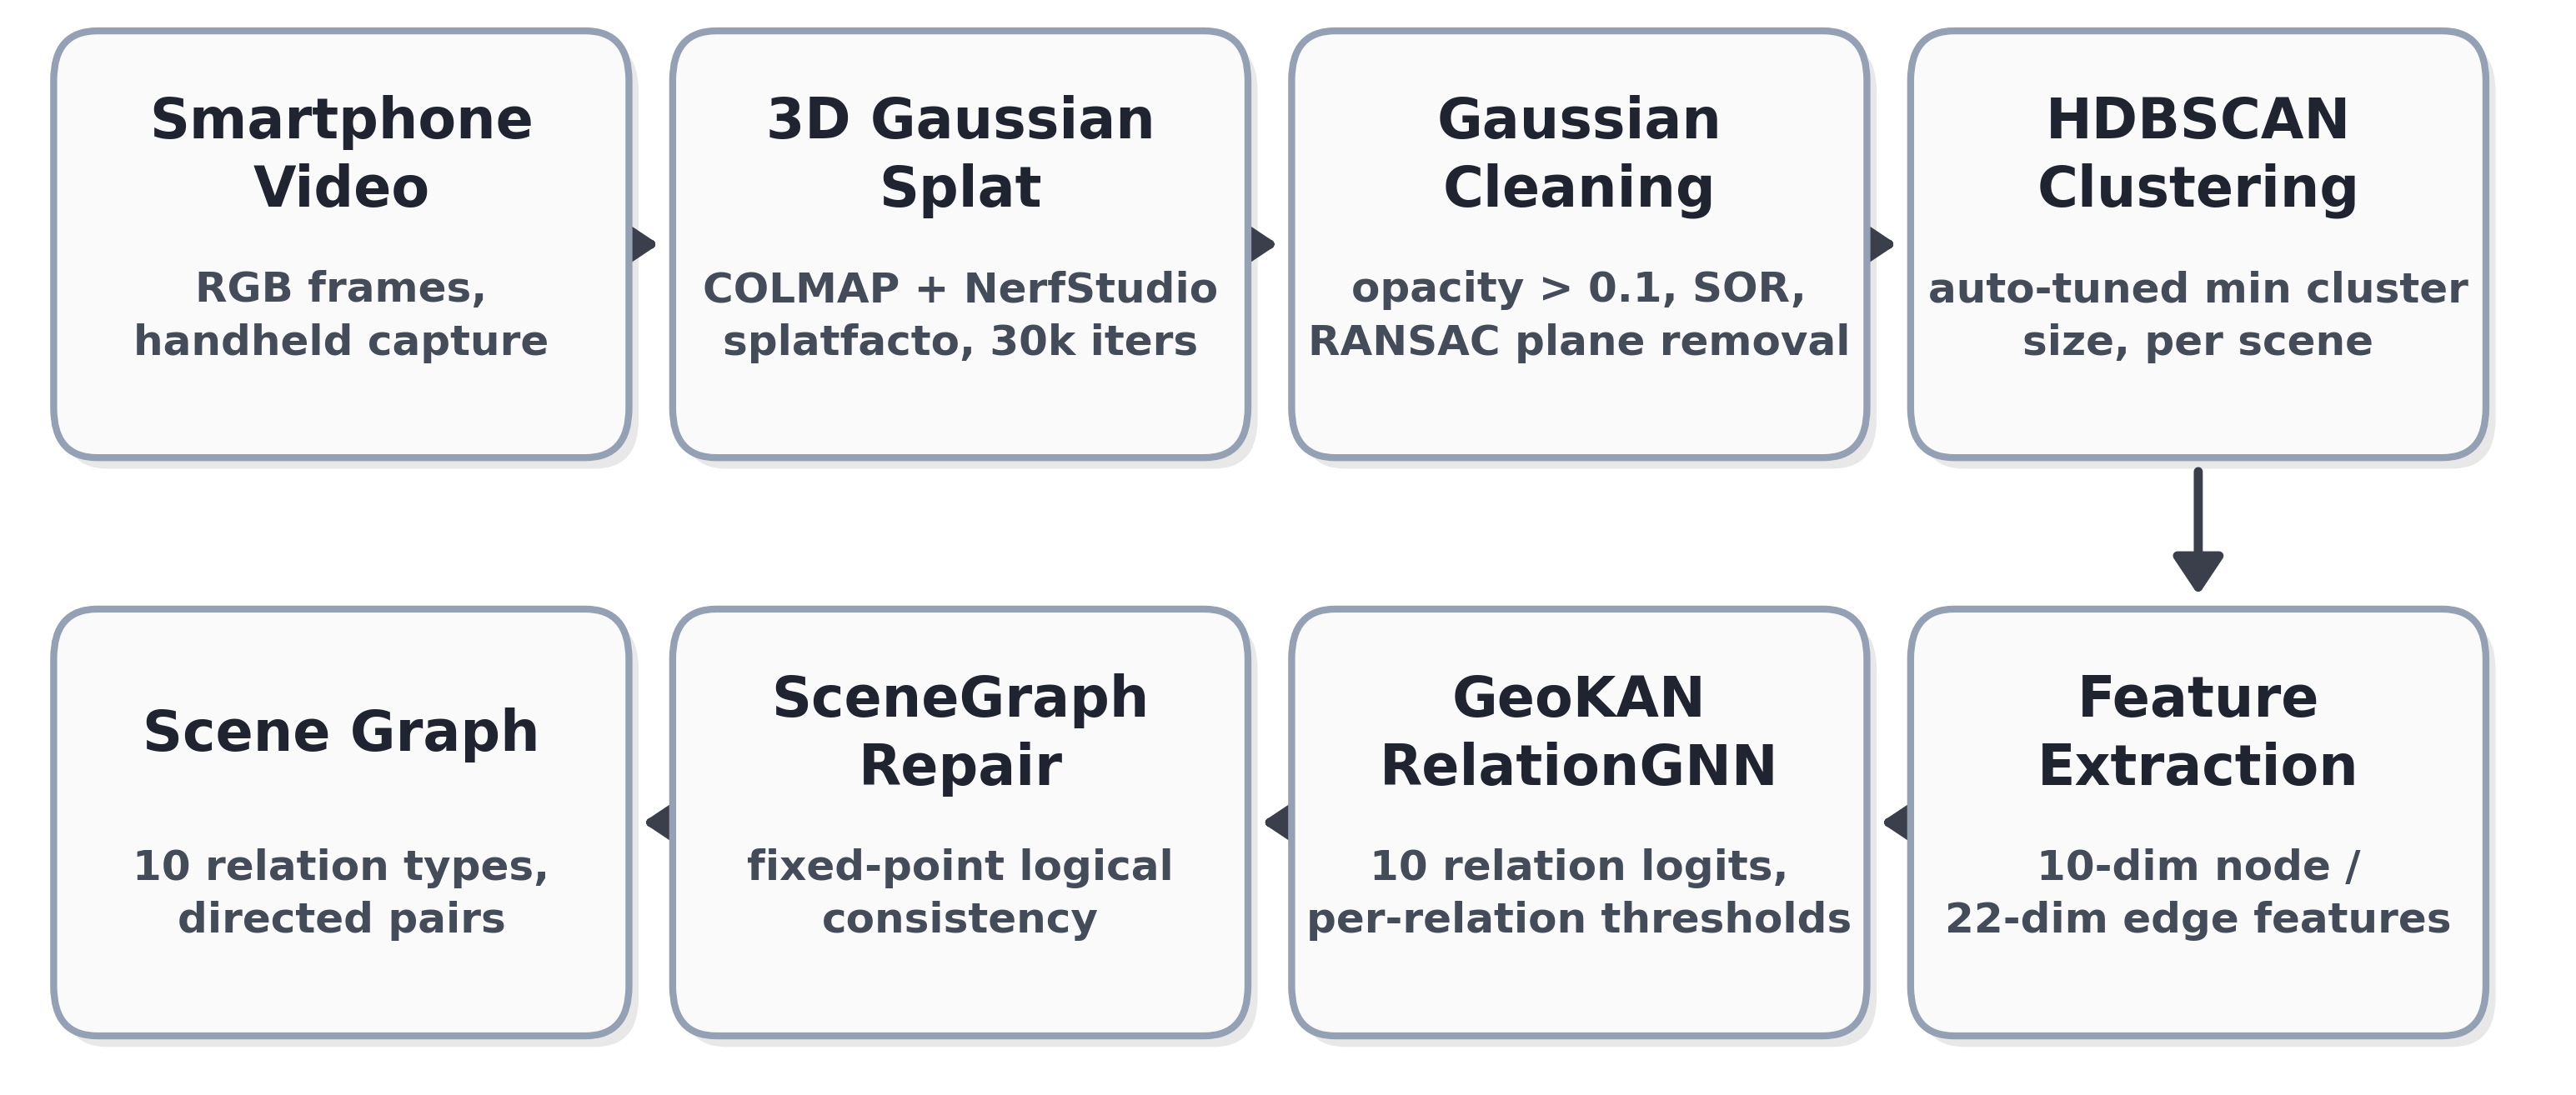
\includegraphics[width=\textwidth]{figures/fig1_pipeline.png}
\caption{The LogicSplat pipeline, from smartphone video to scene graph.}\label{fig1}
\end{figure}

\FloatBarrier
\subsection{Object Clustering (HDBSCAN)}\label{subsec4-2}

The cleaned Gaussian cloud is segmented into discrete object instances using HDBSCAN, operating on a 6-dimensional feature matrix formed by concatenating XYZ position with RGB colour, normalised to $[0,1]$ and weighted by a factor of $w=0.3$ relative to position, then standardised before clustering:

\begin{equation}
f = \left[x,\ y,\ z,\ w\tfrac{r}{255},\ w\tfrac{g}{255},\ w\tfrac{b}{255}\right], \quad w = 0.3
\label{eq:clusterfeat}
\end{equation}

An Otsu saturation threshold is applied beforehand to suppress achromatic background Gaussians; if fewer than 5\% of Gaussians pass this filter, the threshold is halved and reapplied, and disabled entirely if still insufficient, preventing the filter from discarding valid data in scenes with predominantly grey or white objects.

The key clustering parameter, the minimum cluster size, is auto-tuned per scene rather than fixed, since Gaussian density varies considerably across scenes and objects. The tuner sweeps a fixed set of divisors of the point count, runs HDBSCAN at each candidate value under two cluster-selection strategies, and selects the configuration producing a cluster count closest to the midpoint of a target range --- four to twelve objects for training scenes, or pinned to the known object count for the oracle-clustering evaluation settings described in Section~\ref{subsec4-9}. The minimum-samples parameter is fixed at three throughout.

\FloatBarrier
\subsection{Feature Engineering}\label{subsec4-3}

\subsubsection{Node Features (10-Dimensional)}\label{subsubsec4-3-1}

Each object instance is represented by a 10-dimensional feature vector computed from its cluster geometry. The first three dimensions encode centroid position in units of the scene's mean object diagonal, clipped to a maximum of eight diagonal-widths from the scene origin; the next three encode shape aspect ratios --- object size divided by its own bounding-box diagonal --- and are therefore scale-invariant:

\begin{equation}
\hat{c}_k = \frac{1}{8}\,\mathrm{clip}\!\left(\frac{c_k - c_k^{\min}}{\bar d},\ 0,\ 8\right), \qquad s_k = \frac{\mathrm{size}_k}{d_{\text{self}}}, \qquad k \in \{x,y,z\}
\label{eq:nodefeat}
\end{equation}

where $\bar d$ is the scene's mean object diagonal and $d_{\text{self}} = \lVert\mathrm{size}\rVert_2$ is the object's own bounding-box diagonal. A seventh dimension is a log-ratio of object volume relative to the scene median volume; an eighth is a height-to-footprint elongation ratio; a ninth is point density. The final dimension is the object's ordinal rank by height among all objects in the scene, normalised to the unit interval --- a feature that discards all metric information by design, retaining only relative vertical ordering, which is exactly invariant to scene scale.

\subsubsection{Edge Features (22-Dimensional)}\label{subsubsec4-3-2}

For each directed object pair, a 22-dimensional edge feature vector is computed, normalised throughout by the mean of the two objects' bounding-box diagonals rather than by absolute scene extent. The first five dimensions encode directional centroid offsets and distances, each following the same diagonal-relative normalisation pattern:

\begin{equation}
\tilde{x}_{AB} = \frac{1}{3}\,\mathrm{clip}\!\left(\frac{x_A - x_B}{\bar d_{AB}},\ -3,\ 3\right), \qquad \bar d_{AB} = \frac{d_A + d_B}{2}
\label{eq:edgenorm}
\end{equation}

where $\bar d_{AB}$ is the mean bounding-box diagonal of the two objects --- the central mechanism enabling cross-domain transfer, since a value of $\tilde x_{AB}=0.33$ means the same thing, roughly one object-width apart, whether the scene is room-scale or tabletop-scale. The next five dimensions encode footprint overlap, volume ratio, height ratio, vertical gap, and a log-scaled size ratio. A further four dimensions provide alternative normalisations of vertical gap together with a composite contact score:

\begin{equation}
\mathrm{contact}(A,B) = \exp\!\left(-\frac{|g_{AB}|}{0.3\,\bar h_{AB}}\right) \cdot \mathrm{overlap}_{xy}(A,B) \cdot \mathbb{1}\!\left[c_A^z > c_B^z\right]
\label{eq:contact}
\end{equation}

where $g_{AB} = \min_A^z - \max_B^z$ is the vertical gap between A's base and B's top and $\bar h_{AB}$ is the mean height of the two objects --- combining proximity, footprint overlap, and vertical ordering into a single confidence value --- and a footprint-overlap measure relative to the supporting object. Three dimensions encode margin signals used by the rule-injection thresholds described in Section~\ref{subsec4-4}. Two dimensions encode three-dimensional volumetric containment and a centroid-inside-bounding-box flag. The final three dimensions encode a vertical-to-horizontal displacement ratio, separating stacked from side-by-side configurations, and per-axis containment fractions.

This diagonal-relative normalisation is the central mechanism enabling cross-domain transfer: a feature value of, say, 0.3 means the same thing --- roughly one-third of an object-width apart --- whether the scene is a room-scale indoor environment or a tabletop, because both are expressed as multiples of their own scene's characteristic object size rather than in absolute metres.

\FloatBarrier
\subsection{Rule-Based Label Injection}\label{subsec4-4}

Human annotators in 3DSSG label only 80--120 directed object pairs per scene, leaving roughly 90\% of geometrically valid pairs unannotated; standard supervised training treats these as negatives, injecting a false-negative signal that suppresses recall for relations a model could otherwise determine from geometry with certainty. Two complementary mechanisms address this.

Inverse label completion corrects a systematic asymmetry in how annotators label pairs: for every human-annotated relation between objects A and B, the inverse relation between B and A is injected at the same confidence as the source annotation, since annotators consistently label a relation from one perspective (for example, on\_top\_of) and rarely its complement (under), which would otherwise receive almost no positive training examples. Human annotations are never overwritten by this step.

Geometric rule injection instead derives pseudo-labels for every unannotated pair directly from object geometry, at a confidence calibrated to how unambiguous each rule actually is. Directional relations are geometric facts with no ambiguity and are injected at full confidence; the two contact relations carry genuine threshold uncertainty around vertical gap and footprint overlap and are injected at reduced confidence accordingly; adjacent\_to uses the strictest proximity threshold of the four, reflecting the annotation inconsistency this relation is prone to. An existing human-annotated or inverse-completed label always takes priority and is never overwritten by an injected rule.

\begin{table}[htbp]
\centering
\caption{Geometric rule injection confidence by relation.}\label{tab3}
\small
\begin{tabular}{@{}p{3.8cm}p{1.6cm}p{4.3cm}@{}}
\toprule
Relation(s) & Injection confidence & Rationale \\
\midrule
left\_of, right\_of, in\_front\_of, behind, higher\_than, lower\_than & 1.00 & Determined unambiguously by relative centroid position \\
\midrule
on\_top\_of, under & 0.75 & Genuine threshold uncertainty (vertical gap, footprint overlap) \\
\midrule
attached\_to & 0.60 & Bounding-box gap heuristic, moderate certainty \\
\midrule
adjacent\_to & 0.55 & Strict proximity threshold limits false positives \\
\botrule
\end{tabular}
\end{table}

\FloatBarrier
\subsection{The GeoKAN Layer}\label{subsec4-5}

The central architectural idea behind GeoKAN \cite{sen2026geokan} is simple: before a feature is expanded into a richer basis, it should first be rescaled along each dimension according to how much that dimension actually matters for the task. A standard radial basis expansion treats every input dimension as equally informative; GeoKAN instead learns a per-dimension scaling --- a diagonal Riemannian metric $g$ --- that stretches the dimensions the network has found useful and compresses the ones it has not, before any basis function is applied. Given a batch-normalised input $u$, the layer warps it into geometry-adapted coordinates

\begin{equation}
z = u \cdot \sqrt{g}
\label{eq:warp}
\end{equation}

then expands each dimension $z_i$ against twelve fixed centres $c_1 \ldots c_{12}$, spread evenly across the normalised input range.

The three variants compared in this work differ in exactly two places within this pipeline: how $g$ is computed, and which basis function expands $z$. The Gamma variant computes $g = \text{softplus}(\gamma)$, where $\gamma$ is a single learnable scalar per input dimension initialised to zero --- an input-independent metric, the same rescaling applied to every sample. The RBF and Wavelet variants instead compute $g = \text{softplus}(\text{MetricNet}(u))$, where MetricNet is a small two-layer network conditioned on the input itself, initialised so the metric starts at exactly 1.0 --- an input-dependent metric that can, in principle, rescale differently for different samples. All three clamp $g$ to $[0.05, 16]$ for training stability.

For basis expansion, the Gamma and RBF variants both use a radial basis function,

\begin{equation}
\phi_k(z_i) = \exp\left(-\gamma_{rbf} \cdot (z_i - c_k)^2\right)
\label{eq:rbf}
\end{equation}

a smooth, strictly positive bump centred at each $c_k$, with the bandwidth $\gamma_{rbf} = \text{softplus}(\beta)$ similarly constrained to be positive by a separate learned scalar $\beta$. The Wavelet variant instead uses a Mexican hat wavelet,

\begin{equation}
\psi_k(z_i) = \left(1 - (z_i - c_k)^2\right) \cdot \exp\left(-\frac{(z_i - c_k)^2}{2}\right)
\label{eq:wavelet}
\end{equation}

which has a positive peak but negative side-lobes --- a sharper, signed response rather than the RBF's smooth positive one. The flattened basis expansion is concatenated with the normalised input $u$ as a skip connection and passed through a linear layer to produce the layer's output. A regularisation term, penalising deviation of the metric from the identity, is added to the training loss throughout (Section~\ref{subsec4-7}):

\begin{equation}
L_{\text{metric}} = \mathrm{mean}\!\left(\log(g)^2\right)
\label{eq:metricreg}
\end{equation}

\begin{table}[htbp]
\centering
\caption{GeoKAN variant comparison.}\label{tab4}
\begin{tabular}{@{}llll@{}}
\toprule
Variant & Metric type & Metric formula & Basis function \\
\midrule
Gamma & Input-independent & $g = \text{softplus}(\gamma)$, init 0 & Radial basis function \\
\midrule
RBF & Input-dependent & $g = \text{softplus}(\text{MetricNet}(u))$ & Radial basis function \\
\midrule
Wavelet & Input-dependent & $g = \text{softplus}(\text{MetricNet}(u))$ & Mexican hat wavelet \\
\botrule
\end{tabular}
\end{table}

\begin{figure}[htbp]
\centering
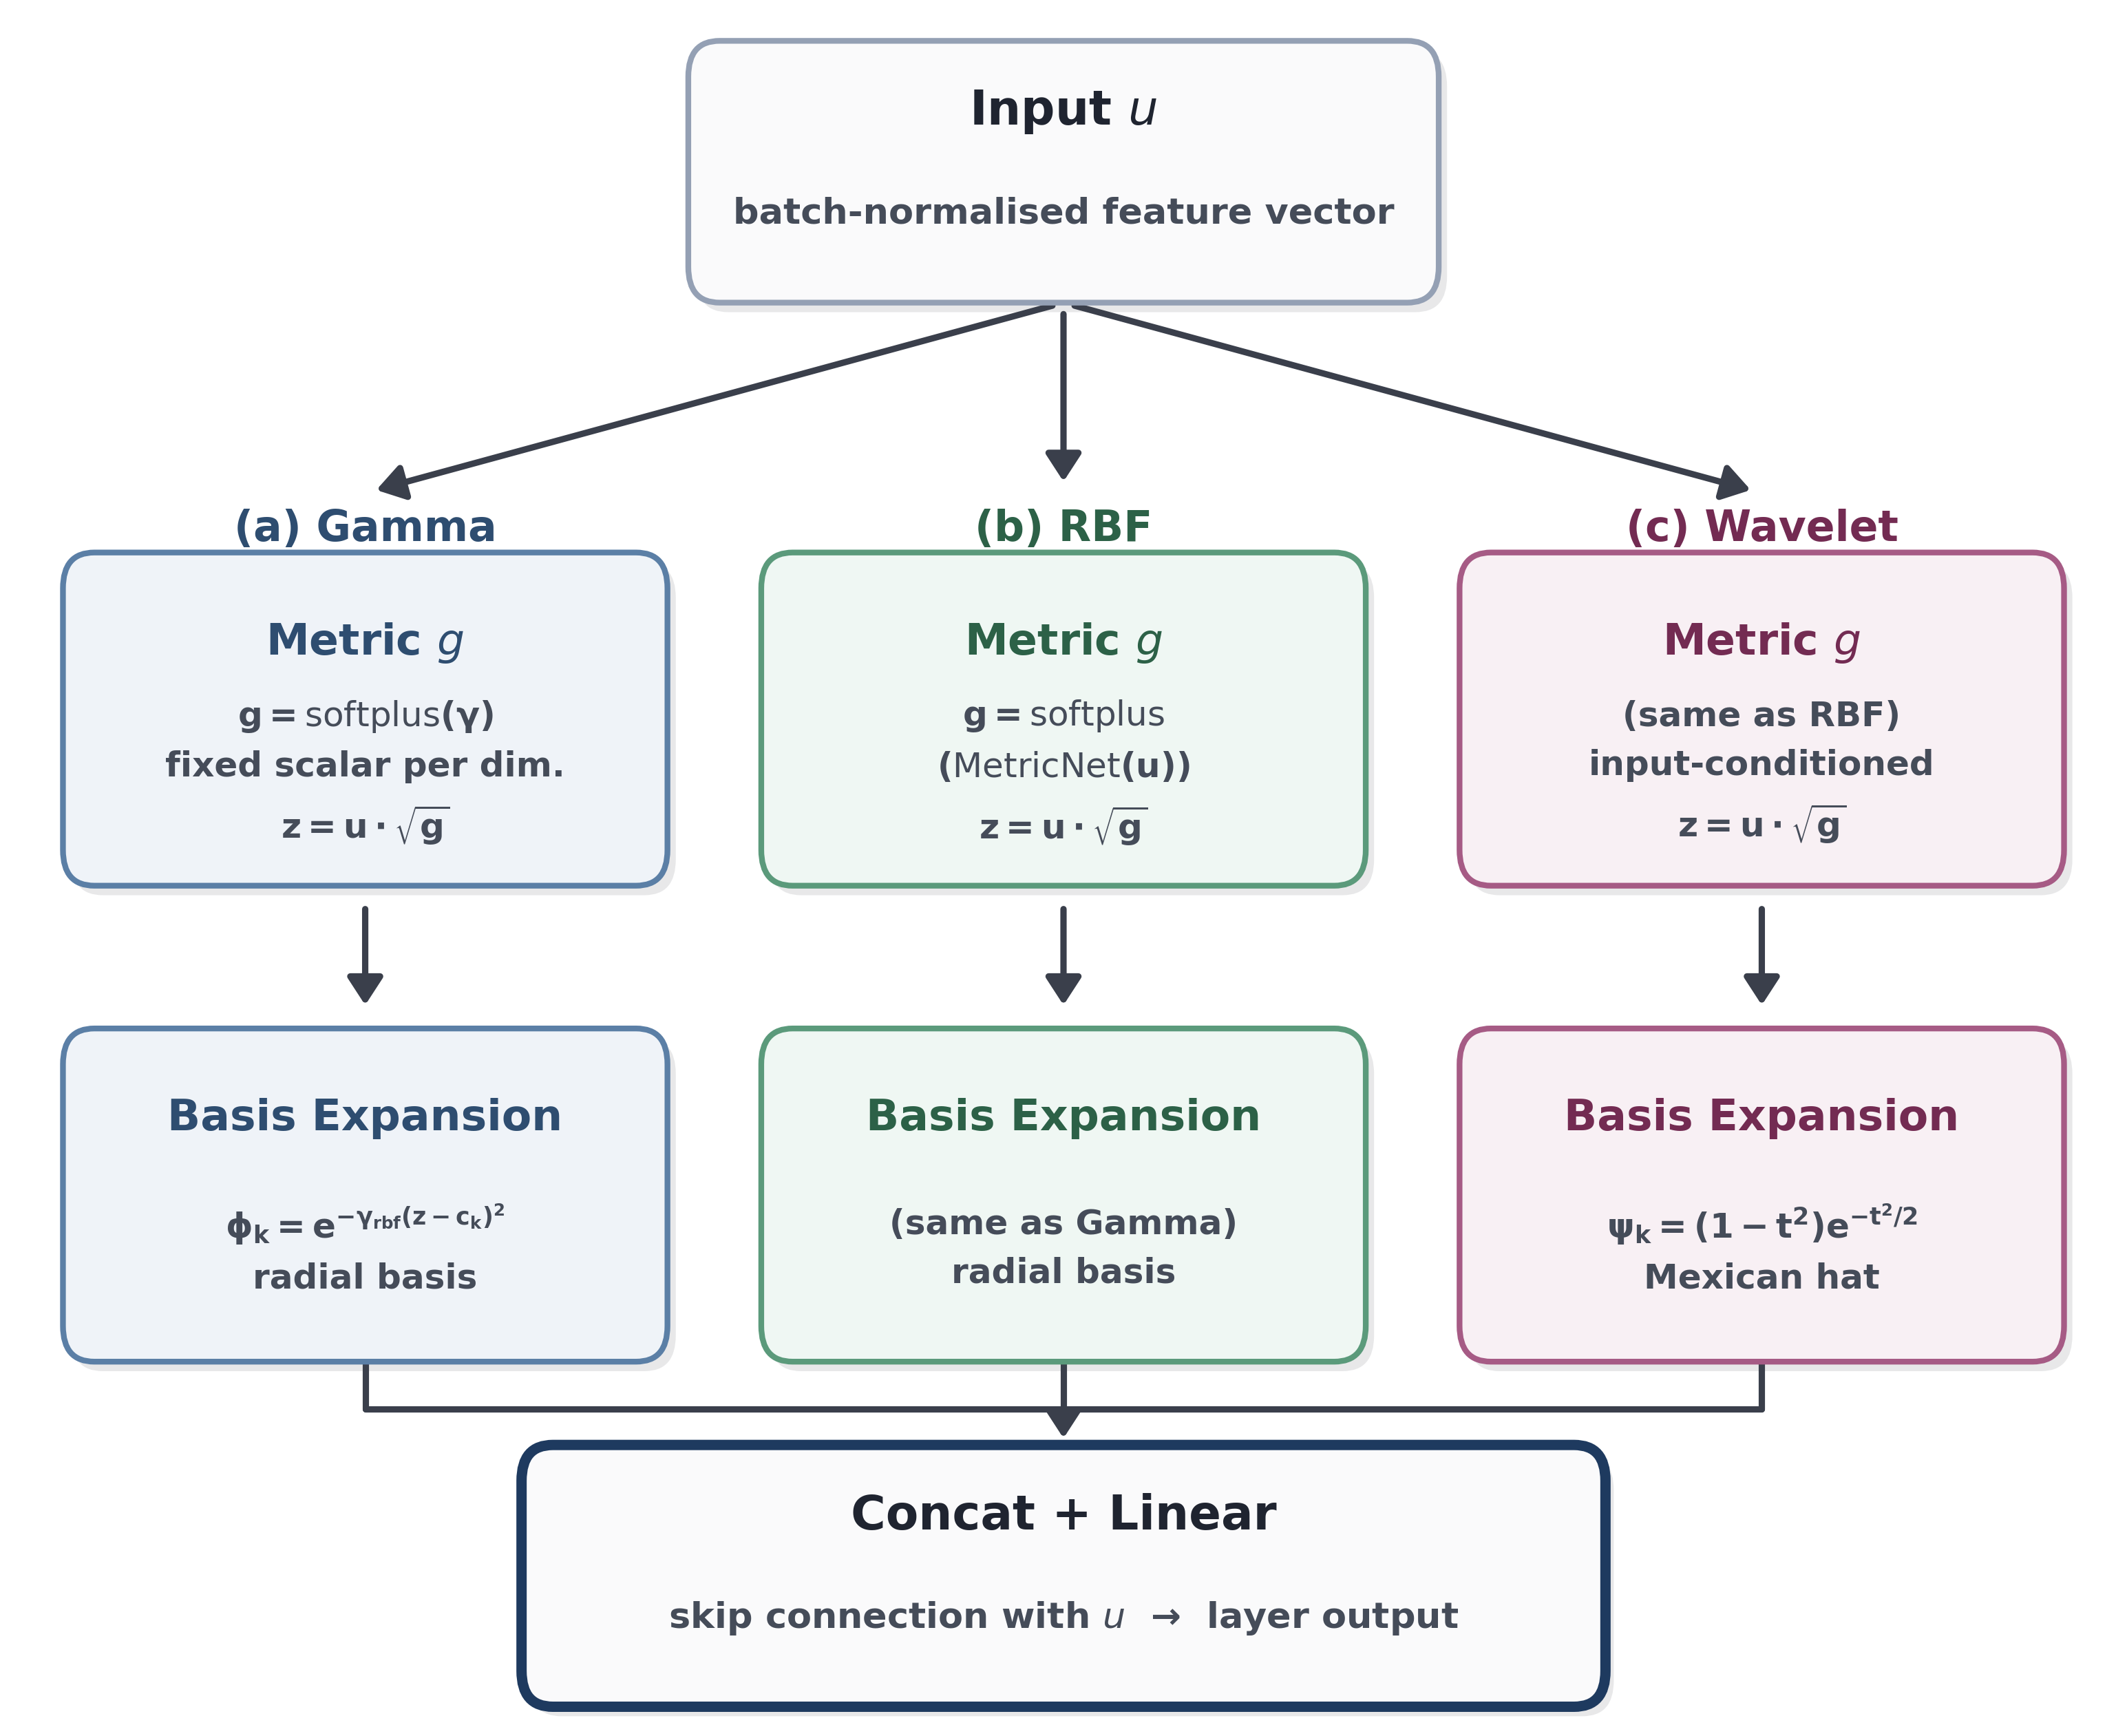
\includegraphics[width=\textwidth]{figures/fig2_geokan_layer.png}
\caption{Internal computation of a single GeoKAN layer, showing where the three variants differ: the metric computation $g$, and the basis function applied after warping.}\label{fig2}
\end{figure}

\FloatBarrier
\subsection{GeoKANRelationGNN Architecture}\label{subsec4-6}

GeoKANRelationGNN converts the per-object node features and per-pair edge features of Section~\ref{subsec4-3} into ten relation logits for every directed object pair, through three stages: graph-context aggregation, pairwise representation construction, and dual-head GeoKAN classification.

The 10-dimensional node feature vector is first projected to a 128-dimensional hidden representation by a single linear layer, followed by layer normalisation and a GELU nonlinearity. Two GATv2Conv layers then aggregate neighbourhood context, each using four attention heads averaged --- rather than concatenated --- back to 128 dimensions, with the 22-dimensional edge feature vector supplied directly to the attention computation so that geometric relationships, not just node identity, shape the attention weights. Each layer is wrapped in a residual connection, ensuring the original geometric signal is never fully overwritten as the network deepens:

\begin{equation}
h \leftarrow \mathrm{LayerNorm}\!\left(\mathrm{GELU}(\mathrm{GATv2Conv}(h)) + h\right)
\label{eq:residual}
\end{equation}

To predict a relation between two specific objects, node-level representations must be combined into a pairwise representation. For each directed pair $(i, j)$, the model forms a 512-dimensional concatenation

\begin{equation}
p_{ij} = \left[h_i,\ h_j,\ h_i - h_j,\ h_i \odot h_j\right]
\label{eq:pairconcat}
\end{equation}

where $\odot$ denotes the elementwise product, and projects it to a 64-dimensional pair embedding via a linear layer, layer normalisation, and GELU. The difference and product terms let this projection learn antisymmetric and conjunctive structure directly, which matters because most of the ten relations are inherently directional: $\text{rel}(i,j)$ and $\text{rel}(j,i)$ are generally not the same relation.

The ten relations are then split across two specialised heads rather than predicted from a single shared classifier. The contact head predicts on\_top\_of, under, attached\_to, and adjacent\_to, and receives the full 22-dimensional edge vector concatenated with the 64-dimensional pair embedding (86 dimensions in total) --- including the vertical-gap, containment, and contact-margin signals needed to judge physical support. The directional head predicts left\_of, right\_of, in\_front\_of, behind, higher\_than, and lower\_than, and receives only the first ten edge dimensions --- centroid offsets, distances, footprint overlap, and basic size ratios --- concatenated with the same pair embedding (74 dimensions in total), since direction is fully determined by relative position alone and the remaining twelve dimensions carry no information relevant to it. Each head is two stacked GeoKAN layers (Section~\ref{subsec4-5}) followed by a linear output layer; the two heads' outputs are concatenated to produce the schema-ordered ten-dimensional logit vector for each directed pair.

\begin{table}[htbp]
\centering
\caption{Dual-head input/output specification.}\label{tab5}
\small
\begin{tabular}{@{}p{1.5cm}p{1.5cm}p{2.4cm}p{1.5cm}p{3cm}@{}}
\toprule
Head & Pair embedding & Edge features used & Total input dim & Relations (n) \\
\midrule
Contact & 64 & All 22 dims & 86 & on\_top\_of, under, attached\_to, adjacent\_to (4) \\
\midrule
Directional & 64 & First 10 dims (position/distance/overlap) & 74 & left\_of, right\_of, in\_front\_of, behind, higher\_than, lower\_than (6) \\
\botrule
\end{tabular}
\end{table}

Across the three basis-function variants, this architecture totals 1,018,414 parameters (Gamma), 1,071,918 (RBF), and 1,071,914 (Wavelet) --- all variants within 0.005\% of one another, the entire difference attributable to the presence or absence of the MetricNet (Section~\ref{subsec4-5}). Every reported configuration uses under 1.1 million parameters in total, roughly three orders of magnitude fewer than the foundation-model-based systems introduced in Section~\ref{sec1}. Section~\ref{subsec4-10} describes a controlled ablation that replaces the GeoKAN layer inside this otherwise unchanged architecture with a conventional learned alternative, isolating the layer's specific contribution from the feature design and training strategy surrounding it.

\begin{figure}[htbp]
\centering
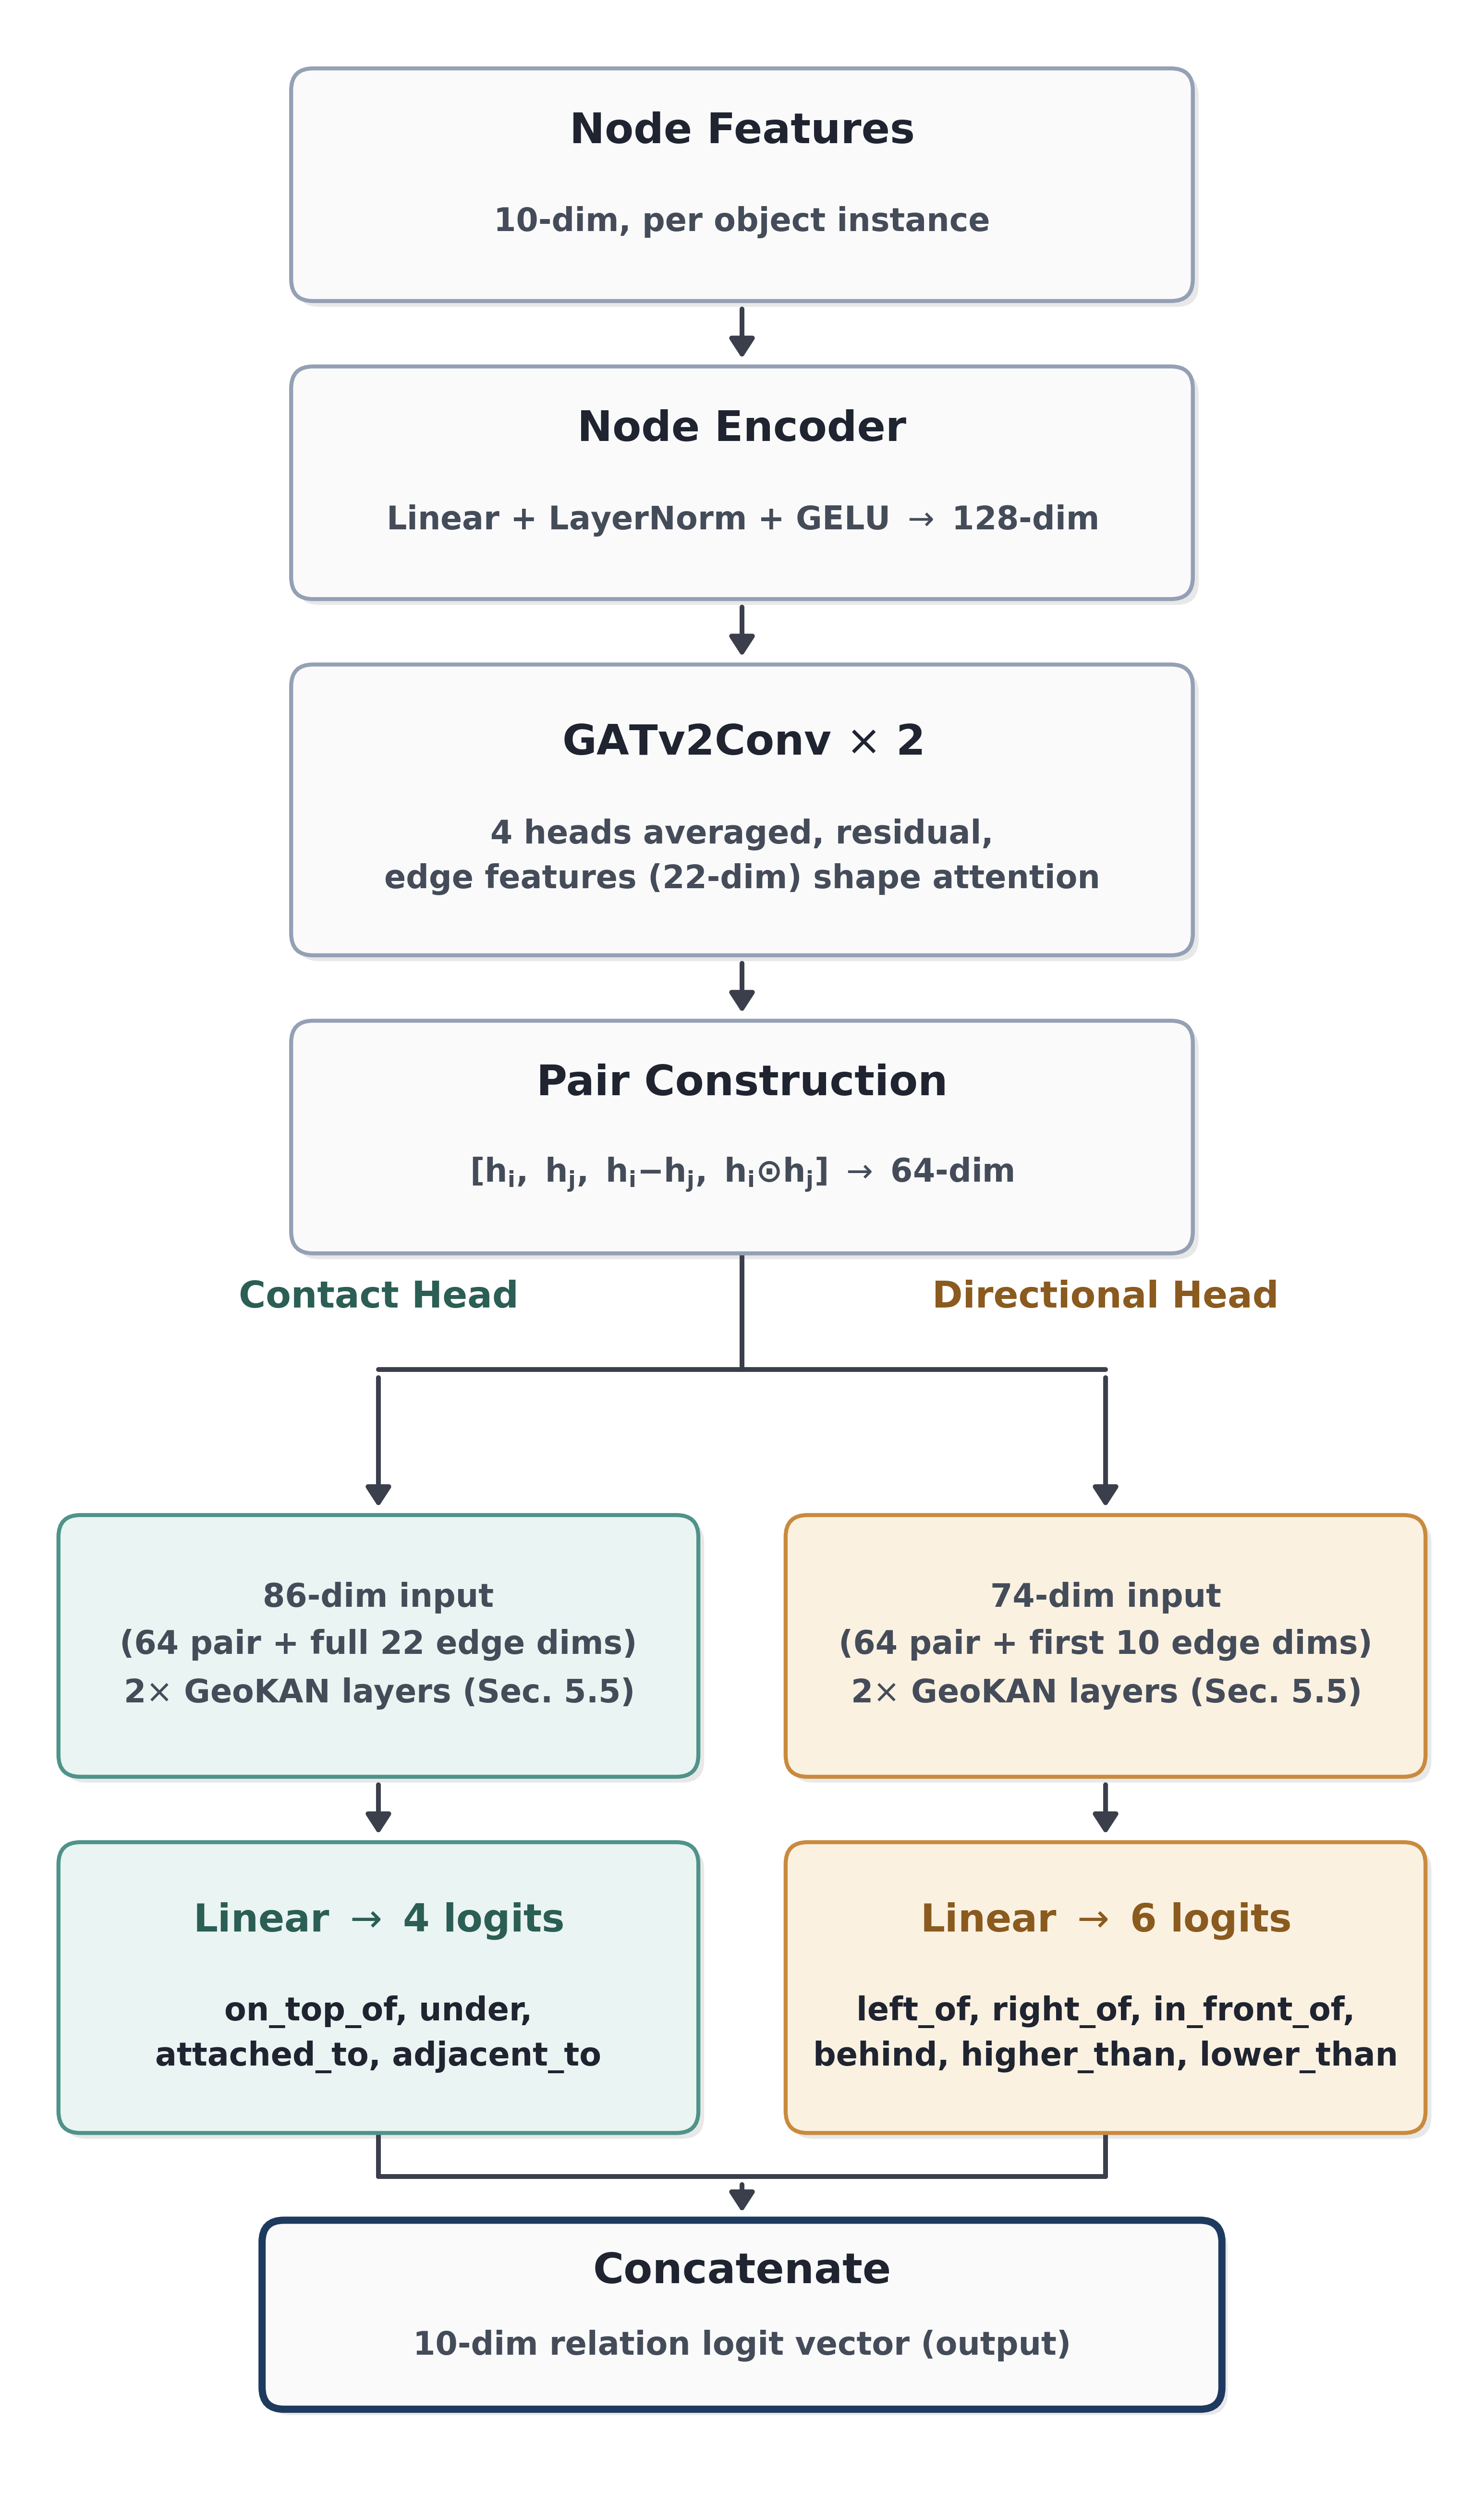
\includegraphics[width=\textwidth]{figures/fig3_dualhead_architecture.png}
\caption{GeoKANRelationGNN architecture: the shared GATv2Conv backbone and pair projection, followed by the dual contact/directional classification heads.}\label{fig3}
\end{figure}

\FloatBarrier
\subsection{Training Strategy}\label{subsec4-7}

All three GeoKAN variants are trained under identical optimisation settings, with one deliberate exception (Gamma's learning rate, below); only the GeoKAN layer's metric and basis function (Section~\ref{subsec4-5}) differ between them.

\textbf{Composite loss.} The primary training signal is an Asymmetric Loss \cite{ridnik2021asl}, chosen because the dominant class --- even after rule-based injection (Section~\ref{subsec4-4}) --- remains the absence of a relation, given that only a small fraction of the roughly 870 possible directed pairs per scene are ever positive. ASL applies a strong focusing parameter to negative examples ($\gamma^-=4.0$) and none to positives ($\gamma^+=0.0$), so confidently correct negatives contribute almost nothing to the gradient while uncertain or incorrect ones still do. Three further mechanisms address different facets of the same imbalance: a per-relation positive-class weight,

\begin{equation}
w_r = \min\!\left(\frac{N_r^-}{N_r^+},\ 8.0\right)
\label{eq:posweight}
\end{equation}

computed as the negative-to-positive label ratio for that relation and capped at 8.0, keeps the rarest relations from being numerically swamped; a manually set per-relation multiplier upweights the four hardest relations --- attached\_to (1.8), adjacent\_to (1.5), on\_top\_of and under (1.2 each); and per-relation label smoothing, ranging from 0.04 for the most geometrically unambiguous relations to 0.12 for adjacent\_to, softens targets in proportion to how uncertain that relation's rule-injected confidence (Section~\ref{subsec4-4}) already is, so the network is not penalised for predicting a calibrated probability instead of a hard 0 or 1.

Two additional terms operate independently of relation identity. An inverse-consistency term penalises disagreement between a relation predicted on one directed edge and its inverse predicted on the reverse edge --- for example, on\_top\_of(A,B) against under(B,A) --- as the mean squared difference between the two probabilities across the four invertible relation pairs $\mathcal{P} = \{(\text{on\_top\_of}, \text{under}), (\text{higher\_than}, \text{lower\_than}), (\text{left\_of}, \text{right\_of}), (\text{in\_front\_of}, \text{behind})\}$:

\begin{equation}
L_{\text{inv}} = \frac{1}{|\mathcal{P}|} \sum_{(R, R^{-1}) \in \mathcal{P}} \left(p_{R(A,B)} - p_{R^{-1}(B,A)}\right)^2
\label{eq:invloss}
\end{equation}

A metric-regularisation term, summed across all four GeoKAN layers in both heads (Section~\ref{subsec4-5}), penalises the squared logarithm of the learned metric $g$ (Equation~\ref{eq:metricreg}), pulling it back toward the identity warp whenever the data gives no strong reason to deviate from it. Formally,

\begin{equation}
L = L_{\text{ASL}} + 0.1 \cdot L_{\text{inv}} + \lambda \cdot L_{\text{metric}}, \quad \lambda = 1\times10^{-4}
\label{eq:loss}
\end{equation}

the three terms are summed directly with no further balancing.

\textbf{Negative edge subsampling.} Independently of the loss weighting above, every training batch is rebalanced before the forward pass: all positive edges are retained, and negative edges are randomly subsampled so that positives make up 30\% of the batch --- addressing the imbalance at the data level, not only at the loss level.

\textbf{Optimisation and schedule.} All variants are trained with AdamW for up to 100 epochs, gradients clipped to a maximum norm of 2.0, with early stopping after 15 epochs without validation F1 improvement. The learning rate follows a linear warmup, then cosine decay to zero over the remaining epochs. The RBF and Wavelet variants use a peak learning rate of $2\times10^{-3}$ with a 5-epoch warmup; the Gamma variant --- whose metric is a single scalar per dimension rather than a full MetricNet --- uses a lower peak rate of $5\times10^{-4}$ with an extended 10-epoch warmup, which was found necessary to keep the scalar metric from oscillating early in training, before the rest of the network has stabilised.

\textbf{Data augmentation.} The training set is expanded sevenfold per scene through six geometric transforms --- rotation by $90^\circ$, $180^\circ$, and $270^\circ$ about the vertical axis, mirroring along each horizontal axis, and small Gaussian jitter of object centroids --- with node features, edge features, and relation labels all transformed consistently under each operation. Scenes containing at least one instance of the rarest relations receive two further mirrored copies beyond this sevenfold expansion, a second, targeted oversampling mechanism layered on top of the per-relation loss weighting above.

\textbf{Threshold calibration.} Once training converges, a per-relation decision threshold is selected by sweeping $[0.10, 0.90]$ in steps of 0.05 on the validation set and keeping the value maximising that relation's F1 --- rather than a single global threshold of 0.5 --- since the ten relations differ substantially in base rate and calibration. These tuned thresholds are then fixed for the evaluation reported in Section~\ref{sec5}.

\begin{table}[htbp]
\centering
\caption{Training hyperparameters (shared across all variants unless noted).}\label{tab6}
\begin{tabular}{@{}ll@{}}
\toprule
Hyperparameter & Value \\
\midrule
Optimizer & AdamW (weight decay $1\times10^{-4}$) \\
\midrule
Learning rate & $2\times10^{-3}$ ($5\times10^{-4}$ for Gamma) \\
\midrule
Warmup & 5 epochs (10 for Gamma), then cosine decay \\
\midrule
Maximum epochs & 100, early stopping with patience 15 \\
\midrule
Batch size & 8 scene graphs per batch \\
\midrule
Gradient clipping & Max norm 2.0 \\
\midrule
Negative edge subsampling & 30\% target positive rate per batch \\
\midrule
Positive-class weight cap & 8.0 \\
\midrule
Data augmentation & $\times$7 (6 geometric transforms + original) \\
\midrule
Metric regularization weight ($\lambda$) & $1\times10^{-4}$ \\
\botrule
\end{tabular}
\end{table}

\FloatBarrier
\subsection{Symbolic Consistency Repair}\label{subsec4-8}

Predictions from GeoKANRelationGNN are made independently for every directed object pair and are not guaranteed to respect the logical structure spatial relations actually obey --- a model may predict on\_top\_of(A,B) without the symmetric under(B,A) ever surfacing, or predict higher\_than(A,B) and higher\_than(B,A) for the same pair simultaneously. SceneGraphRepair removes such contradictions and completes logically implied relations through a deterministic, parameter-free constraint-propagation procedure applied once per scene, after inference.

Four constraint types are enforced, each derived directly from the geometric semantics of the ten relations rather than learned from data. Inverse completeness links four pairs of relations whose direction reverses across the same edge --- on\_top\_of with under, higher\_than with lower\_than, left\_of with right\_of, and in\_front\_of with behind --- so that if one holds between A and B, its inverse should hold between B and A. Mutual exclusion forbids two specific relations from holding in the same direction for the same pair: on\_top\_of(A,B) and under(A,B) cannot both be true, nor can on\_top\_of(A,B) coincide with lower\_than(A,B), since an object resting on top of another cannot simultaneously be vertically lower than it; the same logic applies to the inverse case (under and higher\_than), and independently to the two directional pairs, left\_of/right\_of and in\_front\_of/behind. Asymmetry forbids a relation and its own mirror image from holding at once --- on\_top\_of(A,B) and on\_top\_of(B,A) cannot both be true --- across all eight directional and vertical relations. Transitivity propagates chains: if higher\_than(A,B) and higher\_than(B,C) both hold, higher\_than(A,C) is logically implied, and a direct prediction contradicting that implication signals an error somewhere in the chain. Adjacent\_to is treated separately as a symmetric relation, implying its own reverse rather than a distinct inverse; attached\_to, lacking a natural directional counterpart, is left unconstrained by any of the four mechanisms.

\begin{table}[htbp]
\centering
\caption{The four logical constraint types enforced by symbolic repair.}\label{tab7}
\small
\begin{tabular}{@{}p{2cm}p{2.8cm}p{3.2cm}p{2.3cm}@{}}
\toprule
Constraint & Formal pattern & Action on violation & Example \\
\midrule
Inverse completeness & $R(A,B) \Rightarrow R^{-1}(B,A)$ & Add missing inverse at $0.95\times$ confidence & on\_top\_of $\leftrightarrow$ under \\
\midrule
Mutual exclusion & $R_1(A,B)$ and $R_2(A,B)$ cannot both hold & Remove the lower-confidence relation & on\_top\_of vs. lower\_than \\
\midrule
Asymmetry & $R(A,B)$ and $R(B,A)$ cannot both hold & Remove the lower-confidence relation & higher\_than(A,B) vs. higher\_than(B,A) \\
\midrule
Transitivity & $R(A,B)$ and $R(B,C) \Rightarrow R(A,C)$ & Add implied relation ($\times0.9$) or remove the weaker of chain/contradiction & higher\_than chains \\
\botrule
\end{tabular}
\end{table}

Repair proceeds in two alternating phases, repeated until neither phase changes anything --- a fixed point --- or for a maximum of ten iterations. The removal phase scans every same-direction pair for mutual-exclusion violations and every relation for asymmetry violations, discarding the lower-confidence of the two conflicting predictions in each case; on an exact confidence tie, removal defaults deterministically to one of the two rather than to any meaningful tie-break. It also checks every two-hop transitive chain against the relation directly predicted between its endpoints, removing whichever is less confident --- the chain's weakest link, or the direct contradiction. The addition phase then inserts any inverse, symmetric, or transitively implied relation the removal phase did not already produce, each added at a fraction of the confidence supporting it, so an inferred relation is never reported with higher confidence than the prediction it was inferred from:

\begin{equation}
\mathrm{conf}\!\left(R^{-1}(B,A)\right) = 0.95 \cdot \mathrm{conf}\!\left(R(A,B)\right)
\label{eq:repairinv}
\end{equation}

\begin{equation}
\mathrm{conf}\!\left(R(A,C)\right) = 0.9 \cdot \min\!\left(\mathrm{conf}(R(A,B)),\ \mathrm{conf}(R(B,C))\right)
\label{eq:repairtrans}
\end{equation}

for inverse/symmetric completion and transitive closure respectively, where Equation~\ref{eq:repairtrans} adds the implied relation $R(A,C)$ at $0.9\times$ the weaker of the two chain edges. Because removing a relation can newly enable an addition, and an addition can newly create a contradiction, the two phases are interleaved rather than run once each; in practice, the great majority of scenes converge within two or three iterations.

This mechanism operates entirely on the predicted relation set, never inspects object geometry directly, and is applied identically across all three evaluation settings in Section~\ref{sec5} --- in-domain, held-out LERF, and cross-domain tabletop --- without modification. It is best understood as the last of three complementary mechanisms enforcing the same logical structure at increasing distance from training: rule-based inverse label injection (Section~\ref{subsec4-4}) supplies the signal directly into the training data; the inverse-consistency loss term (Section~\ref{subsec4-7}) penalises disagreement during training; and symbolic repair corrects whatever disagreement remains in the network's predictions at inference time, after the model has otherwise made its decisions independently for each pair.

\FloatBarrier
\subsection{Evaluation Protocol}\label{subsec4-9}

Three quantities are reported across the settings introduced in Section~\ref{sec3}: Recall@K, Macro F1, and Micro F1. Recall@K is computed identically in every setting and is what ties the in-domain and held-out results to a common convention.

Recall@K asks, for every ground-truth relation instance, whether the correct relation type appears among the K highest-scoring relations predicted for that specific directed object pair, out of the ten candidates --- the predicate-classification (PredCls) protocol standard in 3D scene graph literature, used here for direct comparability with ReLaGS, RelationField, and ConceptGraphs on 3DSSG and with GaussianGraph on LERF (Section~\ref{sec1}):

\begin{equation}
\mathrm{Recall@K} = \frac{1}{|\mathcal{G}|} \sum_{(i,j,r) \in \mathcal{G}} \mathbb{1}\!\left[r \in \mathrm{top}_K\!\left(\mathrm{scores}_{ij}\right)\right]
\label{eq:recallk}
\end{equation}

where $\mathcal{G}$ is the set of ground-truth $(\text{subject}, \text{object}, \text{relation})$ triples and $\mathrm{top}_K(\mathrm{scores}_{ij})$ is the set of $K$ highest-scoring relation types for pair $(i,j)$. Because it ranks relations rather than thresholding them, Recall@K is threshold-free and is reported alongside, not instead of, the threshold-dependent F1 scores below.

Macro F1, reported for in-domain validation, is the unweighted mean of ten per-relation F1 scores, each computed at that relation's individually tuned decision threshold (Section~\ref{subsec4-7}) over the pairs for which that relation is annotated or rule-injected:

\begin{equation}
\mathrm{Macro\ F1} = \frac{1}{10} \sum_{r=1}^{10} \frac{2\,P_r R_r}{P_r + R_r}
\label{eq:macrof1}
\end{equation}

averaged uniformly across relations rather than across instances, so the rarer relations are not swamped by adjacent\_to and the directional relations, which dominate by raw count. Micro F1, reported for the cross-domain tabletop setting, instead pools true positives, false positives, and false negatives across every relation and every scene into a single precision/recall/F1 calculation:

\begin{equation}
\mathrm{Micro\ F1} = \frac{2 \sum_r \mathrm{TP}_r}{2 \sum_r \mathrm{TP}_r + \sum_r \mathrm{FP}_r + \sum_r \mathrm{FN}_r}
\label{eq:microf1}
\end{equation}

a more stable choice for a benchmark an order of magnitude smaller in scene count, where ten separate per-relation scores per scene would be dominated by sampling noise.

Object instances for the held-out LERF and cross-domain tabletop settings are obtained through oracle clustering: the known object count for each scene is supplied to the HDBSCAN auto-tuner (Section~\ref{subsec4-2}) as an exact target, rather than left for the tuner to infer from the splat alone. This mirrors the PredCls convention itself, which evaluates relation prediction against ground-truth object instances rather than instances produced by an upstream detector --- isolating the quality of relation prediction, the contribution this study is concerned with, from class-agnostic 3D instance segmentation, a separate problem governed entirely by HDBSCAN's own density and cluster-size parameters. In-domain validation does not require this step, since 3RScan scenes carry ground-truth instance segmentation already attached to each Gaussian through nearest-vertex label transfer (Section~\ref{subsec3-1}).

The two consistency mechanisms described in this study contribute unevenly across the three settings, in proportion to how far each sits from the training distribution. In-domain validation --- where rule-injected training labels and the inverse-consistency loss (Section~\ref{subsec4-7}) already resolve most cross-edge contradictions before the network is even evaluated --- applies only a lightweight same-edge correction: resolving the comparatively rare cases where left\_of and right\_of, in\_front\_of and behind, or higher\_than and lower\_than both cross their decision threshold for the same directed pair, by keeping whichever side the network is more confident about. The held-out LERF and cross-domain tabletop settings instead apply the full SceneGraphRepair module (Section~\ref{subsec4-8}) unmodified --- cross-edge inverse completion, asymmetry resolution, and transitive closure included --- and report results both before and after this step, since operating outside the training distribution makes graph-level contradictions in the raw predictions noticeably more frequent, and the full module's contribution correspondingly more visible.

\begin{table}[htbp]
\centering
\caption{Evaluation settings and protocol.}\label{tab8}
\small
\begin{tabular}{@{}p{2.2cm}p{2.4cm}p{2cm}p{3.4cm}@{}}
\toprule
Setting & Object count source & Headline metric(s) & Consistency mechanism before scoring \\
\midrule
In-domain (3DSSG val) & Ground-truth instance segmentation & Macro F1, Recall@3/5 & Same-edge exclusivity only \\
\midrule
Held-out LERF & Oracle clustering & Recall@3/5 (mean) & Full SceneGraphRepair, before/after reported \\
\midrule
Cross-domain tabletop & Oracle clustering & Micro F1, Recall@3/5 & Full SceneGraphRepair, before/after reported \\
\botrule
\end{tabular}
\end{table}

\FloatBarrier
\subsection{Controlled Architecture Ablation}\label{subsec4-10}

To test whether the GeoKAN layer's specific contribution can be separated from the feature design, rule-based injection, and symbolic repair described elsewhere in this section, a matched-budget baseline replaces the GeoKAN layer inside the otherwise identical GeoKANRelationGNN wrapper (Section~\ref{subsec4-6}) with a conventional learned layer. Where GeoKAN warps its input through a learned or fixed metric before expanding it against a fixed basis function (Section~\ref{subsec4-5}), the baseline instead learns the expansion directly: a single linear layer maps the input to the same output width the basis expansion would have produced, followed by GELU and dropout, then the same skip connection and output-mixing layer GeoKAN uses. This keeps the surrounding architecture, training data, augmentation, loss, optimiser, schedule, and threshold-calibration procedure (Sections~\ref{subsec4-6}--\ref{subsec4-9}) completely unchanged --- the only difference is what happens inside the layer. The baseline's learned expansion carries more parameters than GeoKAN's metric step (1,570,666 in total, against 1,018,414 for GeoKAN-Gamma), a deliberate choice to avoid disadvantaging the baseline on capacity; if GeoKAN holds any advantage under this comparison, it is not because the alternative was starved of capacity to compensate. The baseline is trained with the same default learning rate and warmup used for GeoKAN-RBF and GeoKAN-Wavelet (Section~\ref{subsec4-7}), not Gamma's lower, specially-tuned rate, since that adjustment was motivated by a property specific to Gamma's scalar metric rather than a general training instability the baseline would also be expected to need.

\begin{figure}[htbp]
\centering
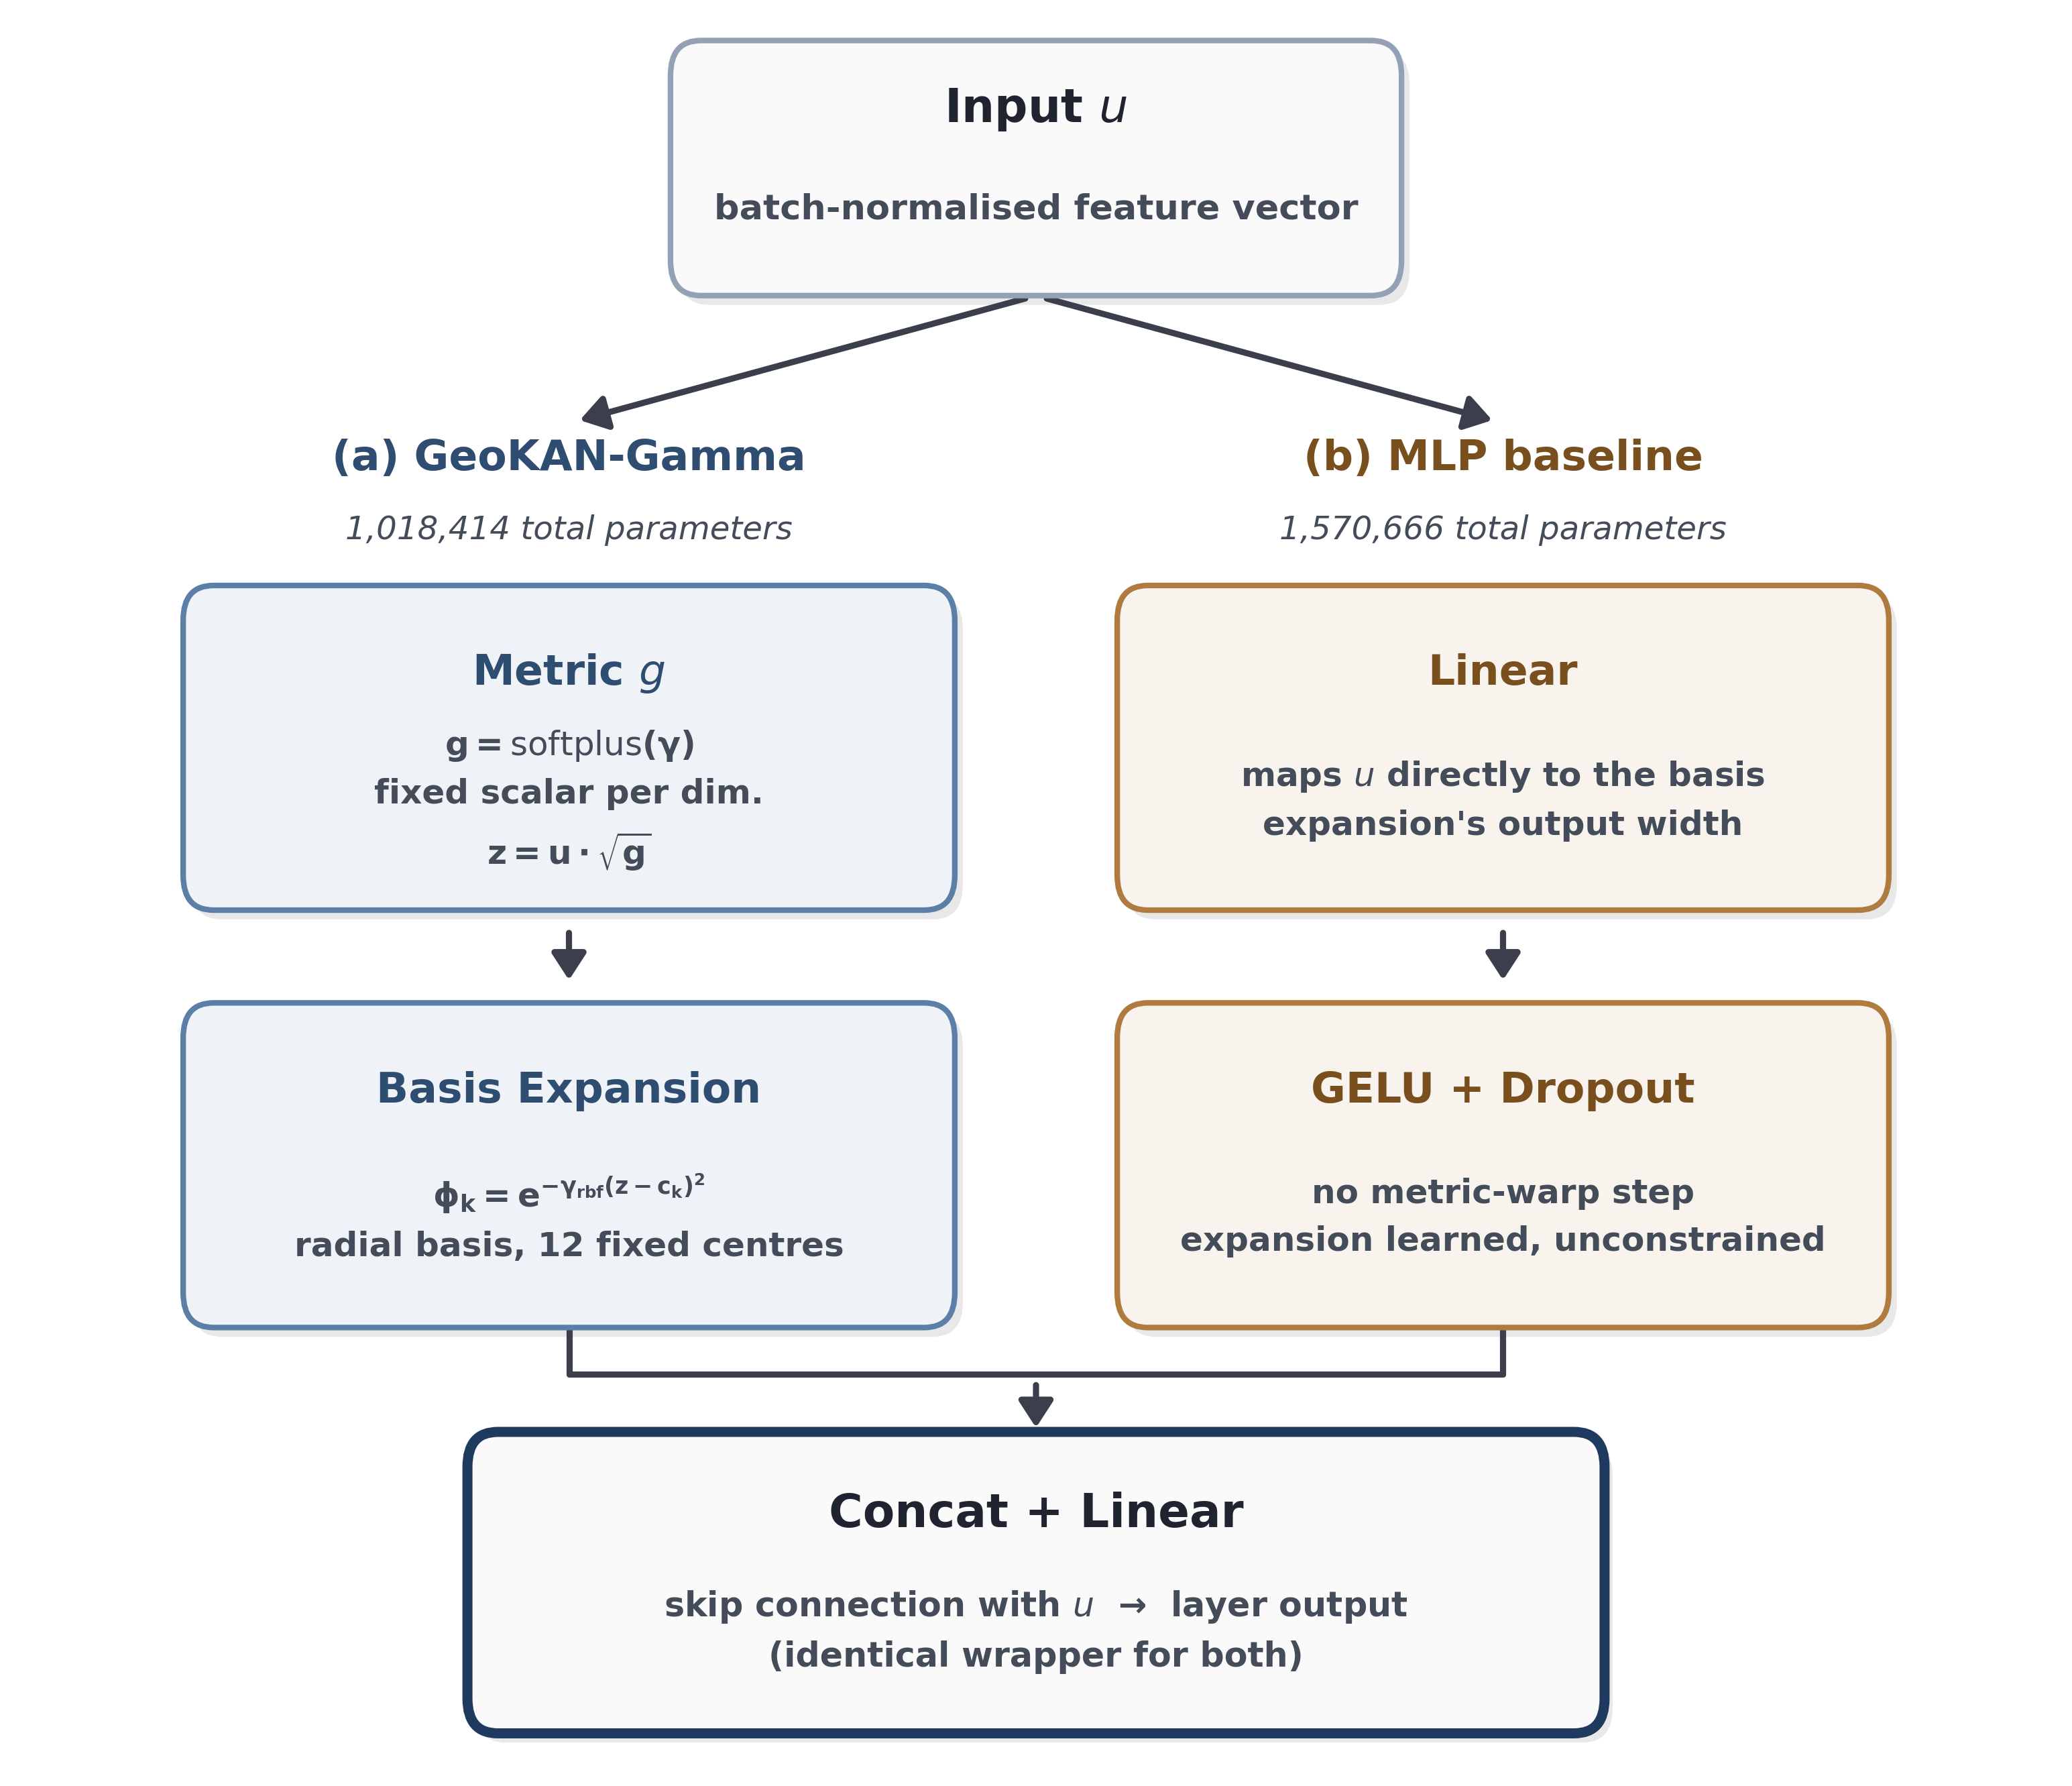
\includegraphics[width=\textwidth]{figures/fig4_mlp_ablation.png}
\caption{Controlled architecture ablation: the GeoKAN layer (Section~\ref{subsec4-5}) replaced by a matched-budget conventional learned layer, with the rest of the architecture (Section~\ref{subsec4-6}) unchanged.}\label{fig4}
\end{figure}

\FloatBarrier
\section{Results and Discussions}\label{sec5}

\FloatBarrier
\subsection{In-Domain Results (3DSSG Validation)}\label{subsec5-1}

\begin{table}[htbp]
\centering
\caption{Architecture comparison on the 3DSSG validation split (85 scenes), tuned per-relation thresholds.}\label{tab9}
\begin{tabular}{@{}lllll@{}}
\toprule
Configuration & Macro F1 & Recall@3 & Recall@5 & Parameters \\
\midrule
MLP baseline & 0.9325 & 0.8783 & 0.9817 & 1,570,666 \\
\midrule
GeoKAN-Gamma & 0.9257 & 0.8779 & 0.9832 & 1,018,414 \\
\midrule
GeoKAN-RBF & 0.9194 & 0.8747 & 0.9818 & 1,071,918 \\
\midrule
GeoKAN-Wavelet & 0.9135 & 0.8716 & 0.9795 & 1,071,914 \\
\botrule
\end{tabular}
\end{table}

In-distribution, the four configurations are close enough that no single one is unambiguously best: the matched-budget MLP baseline reaches the highest Macro F1, GeoKAN-Gamma the highest Recall@5, and the two are nearly identical on Recall@3 (0.8783 versus 0.8779), with GeoKAN-RBF close behind on both rankings. GeoKAN-Wavelet trails on every metric. Within the GeoKAN family specifically, the ordering is consistent across all three metrics --- Gamma exceeds RBF exceeds Wavelet --- despite Gamma's metric being a fixed scalar per dimension rather than the input-conditioned MetricNet the other two use, indicating that an adaptive metric offers no measurable benefit when the input features are already scale-invariant and well-engineered (Section~\ref{subsec4-3}). Against the MLP baseline specifically, GeoKAN shows no in-distribution advantage, consistent with Yu et al.'s broader finding that KAN-style architectures match but do not exceed conventional MLPs outside symbolic-regression tasks (Section~\ref{sec2}) --- the architectural choice that does matter is examined in Section~\ref{subsec5-2} and \ref{subsec5-3}, where the training distribution is left behind. GeoKAN-Gamma is the strongest-performing variant in-distribution on every metric in Table~\ref{tab9} and is carried forward as the representative GeoKAN configuration for the held-out LERF evaluation (Section~\ref{subsec5-3}); the cross-domain tabletop evaluation (Section~\ref{subsec5-2}) instead tests all three GeoKAN variants, since in-distribution ranking turns out not to predict cross-domain ranking.

\begin{table}[htbp]
\centering
\caption{Recall@5 against foundation-model-dependent and per-scene-optimised baselines on 3DSSG. ReLaGS, RelationField, ConceptGraphs, and Open3DSG figures are reproduced from ReLaGS's own Table~1 comparison on 3DSSG, the only published evaluation that benchmarks all four under a matched protocol; not independently re-evaluated here.}\label{tab10}
\begin{tabular}{@{}llp{5cm}@{}}
\toprule
System & Recall@5 & Requirement at inference \\
\midrule
LogicSplat (GeoKAN-Gamma) & 98.3\% & None (1.02M total parameters) \\
\midrule
ReLaGS & 87.0\% & CLIP + SAM ($\sim$1.5B parameters) \\
\midrule
RelationField & 82.0\% & Per-scene optimisation ($\sim$60 min/scene, single A100) \\
\midrule
ConceptGraphs & 79.0\% & Large language model \\
\midrule
Open3DSG & 65.0\% & CLIP \\
\botrule
\end{tabular}
\end{table}

LogicSplat exceeds every compared system by 11 to 33 percentage points, including RelationField, whose per-scene optimisation gives it access to information --- a model fit specifically to the test scene --- that none of the other systems in this table, including LogicSplat, receive.

\FloatBarrier
\subsection{Cross-Domain Tabletop Results}\label{subsec5-2}

\begin{table}[htbp]
\centering
\caption{Zero-shot tabletop result for all three GeoKAN classification-head variants from Table~\ref{tab9} and the matched-budget MLP baseline --- every row below is a LogicSplat configuration; none is an external system. All four are trained on 3RScan only, with no tabletop fine-tuning, oracle clustering, and thresholds carried over unmodified from the 3DSSG validation set.}\label{tab11}
\small
\begin{tabular}{@{}p{1.6cm}p{1.5cm}p{1.1cm}p{1.2cm}p{1cm}p{1.2cm}p{1.2cm}@{}}
\toprule
System & Stage & Micro F1 & Precision & Recall & Recall@3 & Recall@5 \\
\midrule
GeoKAN-Gamma & Before repair & 0.740 & 0.815 & 0.677 & 0.758 & 0.927 \\
\midrule
GeoKAN-Gamma & After repair & 0.774 & 0.773 & 0.776 & 0.758 & 0.927 \\
\midrule
GeoKAN-RBF & Before repair & 0.777 & 0.861 & 0.709 & 0.793 & 0.943 \\
\midrule
GeoKAN-RBF & After repair & 0.802 & 0.841 & 0.768 & 0.793 & 0.943 \\
\midrule
GeoKAN-Wavelet & Before repair & 0.783 & 0.874 & 0.709 & 0.789 & 0.933 \\
\midrule
GeoKAN-Wavelet & After repair & 0.819 & 0.868 & 0.776 & 0.789 & 0.933 \\
\midrule
MLP baseline & Before repair & 0.714 & 0.763 & 0.671 & 0.740 & 0.886 \\
\midrule
MLP baseline & After repair & 0.721 & 0.710 & 0.732 & 0.740 & 0.886 \\
\botrule
\end{tabular}
\end{table}

Recall@3 and Recall@5 are identical before and after repair for every system, since they are computed from raw ranked scores prior to thresholding (Section~\ref{subsec4-9}); repair only modifies the thresholded prediction set, so its effect surfaces in Micro F1, precision, and recall rather than in the ranking metrics. All three GeoKAN variants exceed the matched-budget MLP baseline on every column, by 5.3 to 9.8 Micro F1 points and 4.1 to 5.7 Recall@5 points after repair. Within the GeoKAN family, however, the ranking inverts relative to Table~\ref{tab9}: GeoKAN-Wavelet leads after repair (Micro F1 = 0.819, Recall@5 = 0.933), GeoKAN-RBF is close behind (0.802, 0.943), and GeoKAN-Gamma --- the strongest variant in-distribution --- trails both (0.774, 0.927). This is the first evidence in this study that GeoKAN's architectural choice matters, but in the opposite direction from what in-distribution performance alone would predict: the input-conditioned MetricNet used by RBF and Wavelet, which offered no measurable in-distribution benefit over Gamma's fixed scalar metric (Section~\ref{subsec5-1}), generalises more robustly once the evaluation domain shifts in scale.

Across the 8 scenes and 508 ground-truth relation triples, repair adds 88 relations for GeoKAN-Gamma, 54 for GeoKAN-RBF, and 42 for GeoKAN-Wavelet, removing 0, 8, and 0 respectively, with every variant converging within 2 iterations --- consistent with the broader pattern that, outside the training distribution, the network under-predicts relations it could in principle complete from what it already got right, more often than it actively contradicts itself.

\begin{table}[htbp]
\centering
\caption{Per-relation F1 before and after repair, GeoKAN-Gamma (3RScan-trained thresholds; attached\_to never occurs in this benchmark and is omitted). Shown as a representative worked example; see text for which patterns generalise to GeoKAN-RBF and GeoKAN-Wavelet.}\label{tab12}
\begin{tabular}{@{}lllll@{}}
\toprule
Relation & F1 (before) & F1 (after) & Change & GT count \\
\midrule
on\_top\_of & 0.621 & 0.919 & +0.298 & 38 \\
\midrule
under & 0.932 & 0.919 & -0.013 & 38 \\
\midrule
adjacent\_to & 0.675 & 0.568 & -0.107 & 54 \\
\midrule
left\_of & 0.868 & 0.860 & -0.008 & 52 \\
\midrule
right\_of & 0.800 & 0.860 & +0.060 & 52 \\
\midrule
in\_front\_of & 0.429 & 0.429 & +0.000 & 52 \\
\midrule
behind & 0.308 & 0.429 & +0.121 & 52 \\
\midrule
higher\_than & 0.920 & 0.920 & +0.000 & 85 \\
\midrule
lower\_than & 0.768 & 0.920 & +0.152 & 85 \\
\botrule
\end{tabular}
\end{table}

The largest gains are concentrated in exactly the relations the inverse-completeness and transitivity rules (Section~\ref{subsec4-8}) are designed to recover: on\_top\_of and lower\_than, both originally under-predicted on tabletop's compact, heavily-stacked arrangements, improve by 0.298 and 0.152 respectively once their logically-implied counterparts are added. The lower\_than gain generalises across all three GeoKAN variants (RBF: +0.114; Wavelet: +0.120), confirming this is a property of the repair mechanism rather than a Gamma-specific artefact. The on\_top\_of gain, by contrast, is largest for Gamma specifically because Gamma's pre-repair F1 on this relation (0.621) starts markedly lower than RBF's (0.788) or Wavelet's (0.932) --- repair recovers under-prediction in proportion to how much under-prediction is actually present, and Wavelet in particular has almost none left to recover (F1 change: $-$0.013). The one relation where repair's net effect is negative for every GeoKAN variant is adjacent\_to (Gamma: $-$0.107; RBF: $-$0.007; Wavelet: $-$0.025), which symbolic repair treats as symmetric and therefore mirrors every predicted instance onto its reverse edge automatically (Section~\ref{subsec4-8}); when the original prediction is itself a false positive, this mirroring duplicates the error onto the reverse pair rather than correcting it.

\FloatBarrier
\subsection{Held-Out LERF Results}\label{subsec5-3}

\begin{table}[htbp]
\centering
\caption{Aggregate LERF result (1,644 ground-truth triples across 4 scenes). The first four rows represent the two LogicSplat configurations introduced in Section~\ref{subsec5-1} (GeoKAN-Gamma and the matched-budget MLP baseline), each shown before and after repair; the last two rows are the external system, GaussianGraph, against its own Table V, corrected to its positional-query rows only --- the relations evaluated here (on\_top\_of, left\_of, higher\_than, etc.) are entirely positional, not functional, and GaussianGraph reports the two separately.}\label{tab13}
\small
\begin{tabular}{@{}p{5cm}p{1.4cm}p{1.4cm}p{1.4cm}@{}}
\toprule
Method & Recall@3 & Recall@5 & Micro F1 \\
\midrule
GeoKAN-Gamma (before repair) & 71.5\% & 94.7\% & 90.1\% \\
\midrule
GeoKAN-Gamma (after repair) & 89.9\% & 95.0\% & 90.0\% \\
\midrule
MLP baseline (before repair) & 70.2\% & 91.8\% & 87.4\% \\
\midrule
MLP baseline (after repair) & 88.4\% & 92.8\% & 87.8\% \\
\midrule
GaussianGraph (LLaVA, no 3D correction, positional) & 45.0\% & 49.8\% & -- \\
\midrule
GaussianGraph (LLaVA + 3D correction, positional) & 61.3\% & 63.2\% & -- \\
\botrule
\end{tabular}
\end{table}

Both LogicSplat configurations exceed GaussianGraph's strongest positional configuration by a wide margin --- 28.6 and 31.8 points at Recall@3 and Recall@5 for GeoKAN-Gamma, 27.1 and 29.6 points for the MLP baseline --- confirming that the headline claim against foundation-model-dependent systems does not depend on which classification head is used. Where the two LogicSplat configurations diverge from each other is consistent with Section~\ref{subsec5-2}: GeoKAN-Gamma leads the MLP baseline on every metric, by 2.2 points in Micro F1 and Recall@5 after repair, the same direction and similar magnitude as the tabletop gap, despite this being a dataset shift rather than a scale shift. Repair adds 39 relations for GeoKAN-Gamma and removes none; for the MLP baseline it adds 48 and removes 1 --- the only contradiction either system produces across every evaluation in this study, a small additional signal that GeoKAN's predictions remain more internally consistent outside the training distribution.

\begin{table}[htbp]
\centering
\caption{Per-scene breakdown for GeoKAN-Gamma, the LogicSplat configuration carried forward for this evaluation (Section~\ref{subsec5-1}).}\label{tab14}
\small
\begin{tabular}{@{}p{1.8cm}p{1.1cm}p{1.3cm}p{1.3cm}p{1.2cm}p{1.3cm}p{1.2cm}@{}}
\toprule
Scene & Objects & GT triples & R@3 before & R@3 after & R@5 before & R@5 after \\
\midrule
ramen & 13 & 616 & 74.4\% & 97.4\% & 99.0\% & 99.0\% \\
\midrule
teatime & 10 & 330 & 69.1\% & 77.9\% & 91.5\% & 91.5\% \\
\midrule
waldo\_kitchen & 10 & 334 & 74.6\% & 89.5\% & 93.1\% & 93.7\% \\
\midrule
figurines & 10 & 364 & 65.9\% & 88.5\% & 91.8\% & 92.3\% \\
\botrule
\end{tabular}
\end{table}

Ramen is already near-saturated before repair (Recall@5 = 99.0\%) and gains entirely at Recall@3; teatime gains the least and is the only scene where neither metric reaches the levels seen elsewhere, suggesting its object arrangement produces relations the model ranks correctly less often to begin with, leaving less for repair to recover from a strong base ranking.

\FloatBarrier
\subsection{Qualitative Example}\label{subsec5-4}

This section walks through one tabletop scene end to end --- the captured input (Figure~\ref{fig5}), its 3D reconstruction (Figure~\ref{fig6}), and the predicted, repaired scene graph (Figure~\ref{fig7}) --- the same scene evaluated quantitatively in Section~\ref{subsec5-2}: a router, hair-dryer box, water bottle, watch, and pen arranged on a table.

\begin{figure}[htbp]
\centering
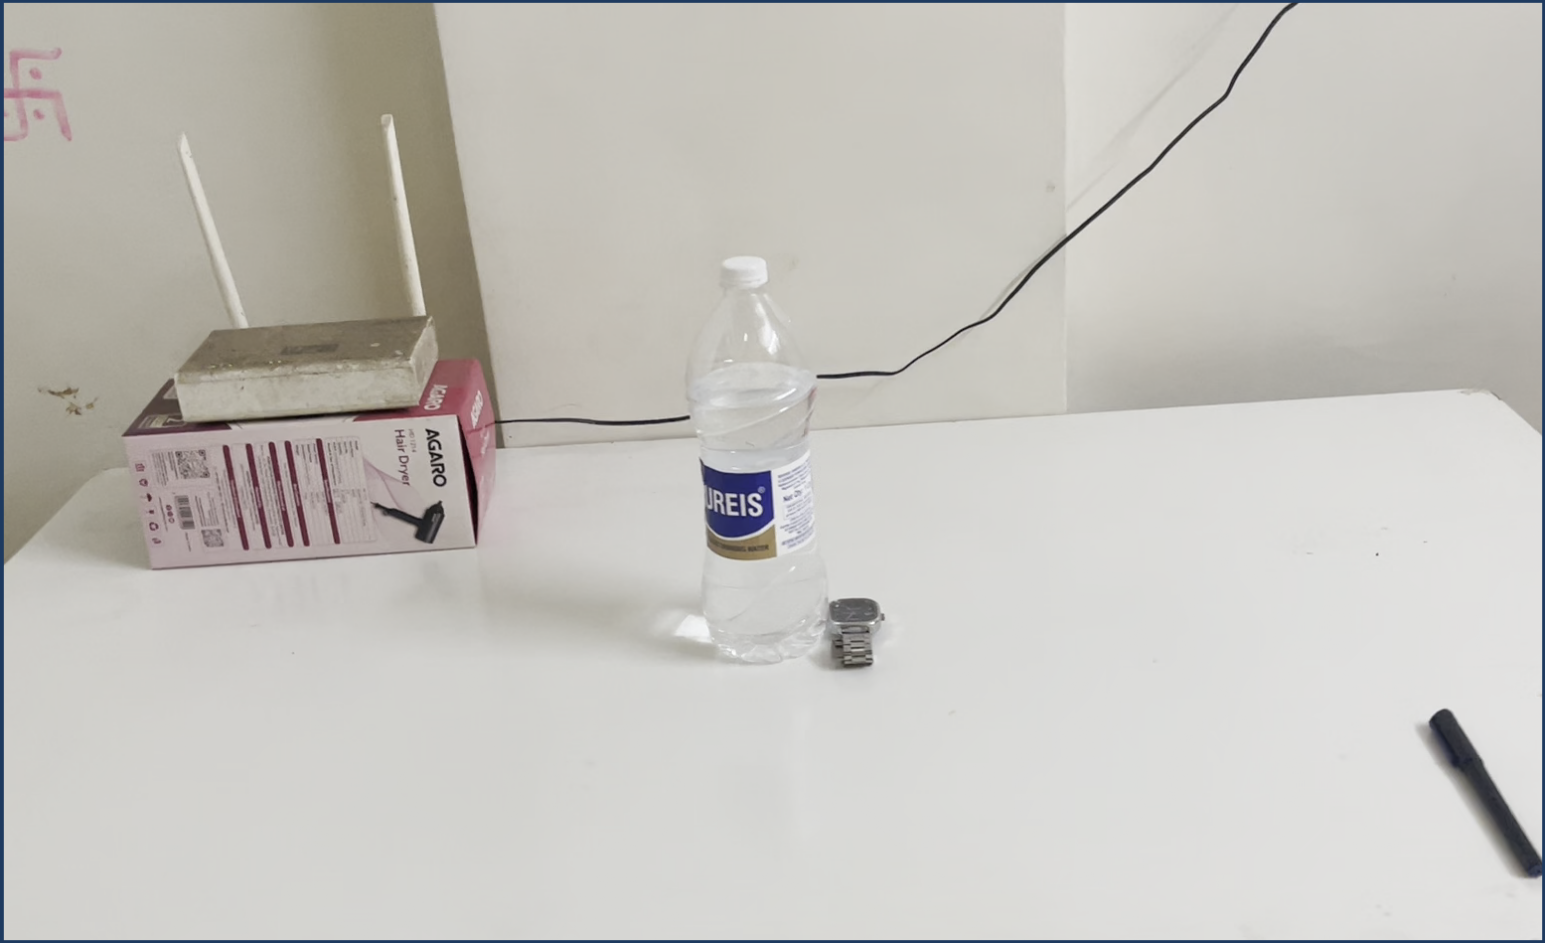
\includegraphics[width=\textwidth]{figures/fig_input_photo.png}
\caption{Sample input frame from the smartphone video of one tabletop scene, prior to 3D reconstruction.}\label{fig5}
\end{figure}

In Figure~\ref{fig6}, the router, hair-dryer box, watch, and water bottle sit close enough together in raw position that colour is what actually separates them in the clustering step itself (Section~\ref{subsec4-2}).

\begin{figure}[htbp]
\centering
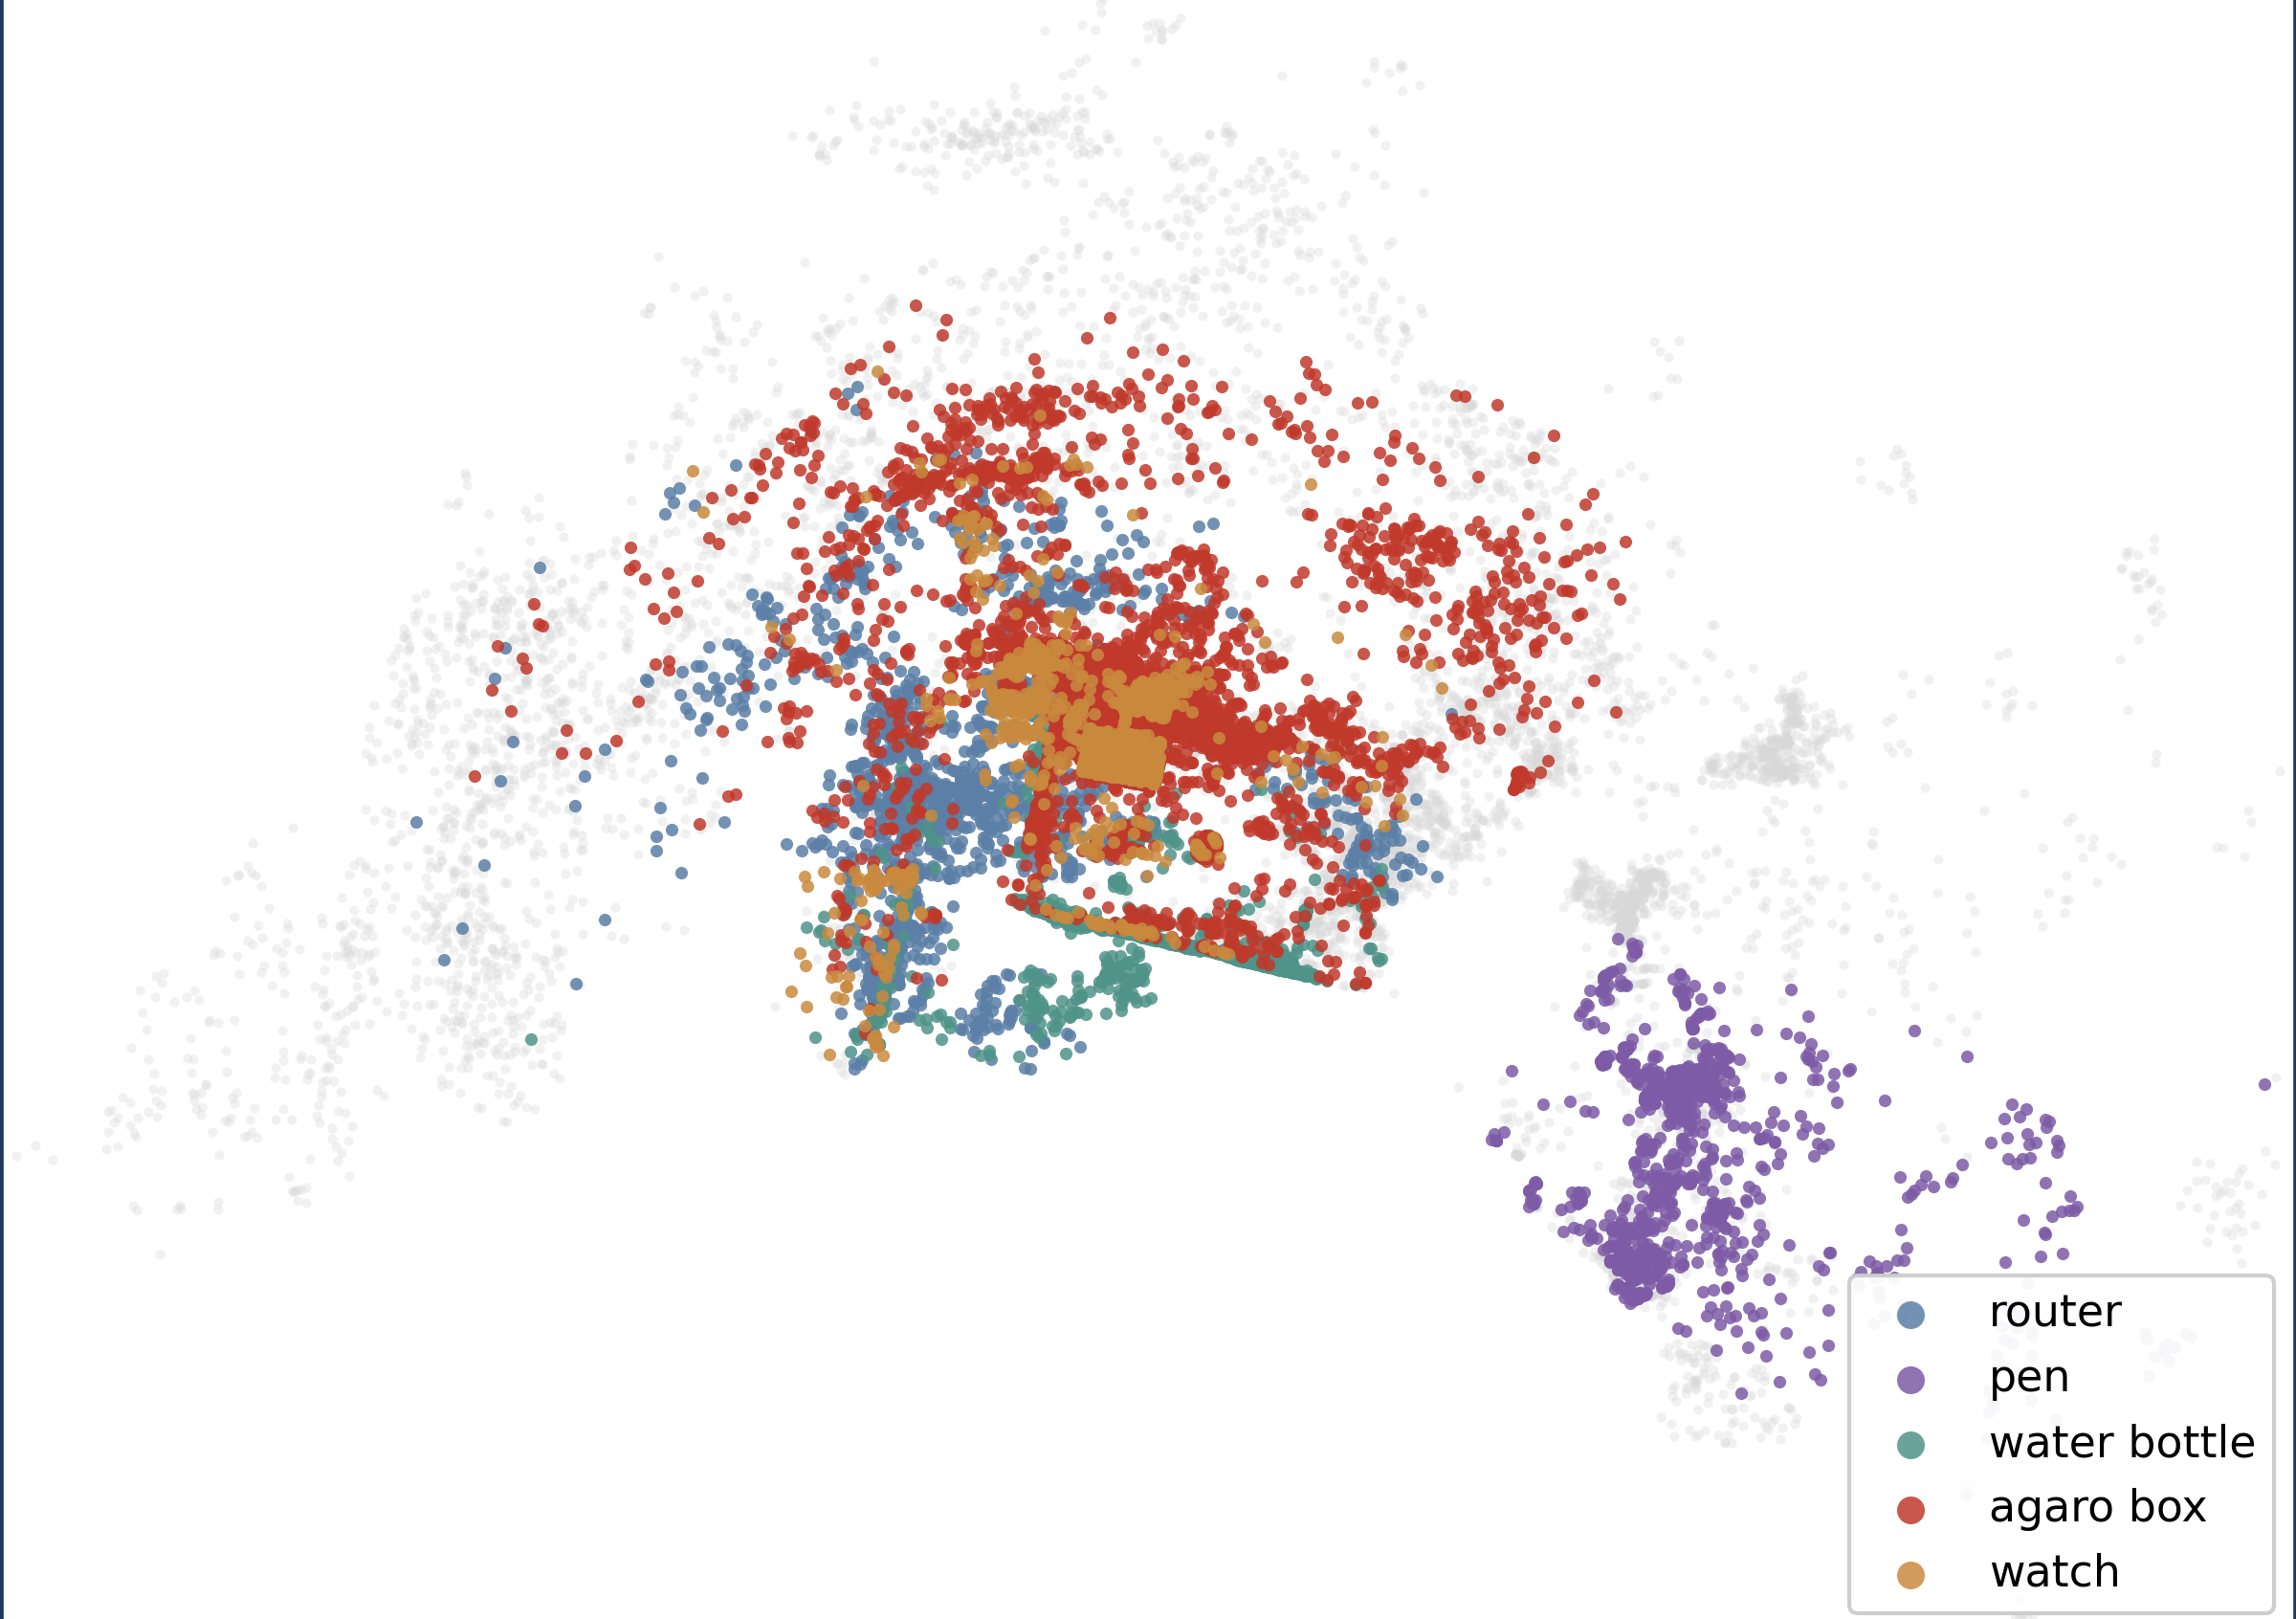
\includegraphics[width=\textwidth]{figures/fig_splat_reconstruction.png}
\caption{Top-down view of the reconstructed 3D Gaussian Splat for the same scene, coloured by per-Gaussian cluster identity (Section~\ref{subsec4-2}) rather than raw splat colour; background and unclustered points shown in grey.}\label{fig6}
\end{figure}

66 of the 84 relations predicted for this scene match ground truth (Figure~\ref{fig7}), consistent with the aggregate accuracy reported in Section~\ref{subsec5-2}.

\begin{figure}[htbp]
\centering
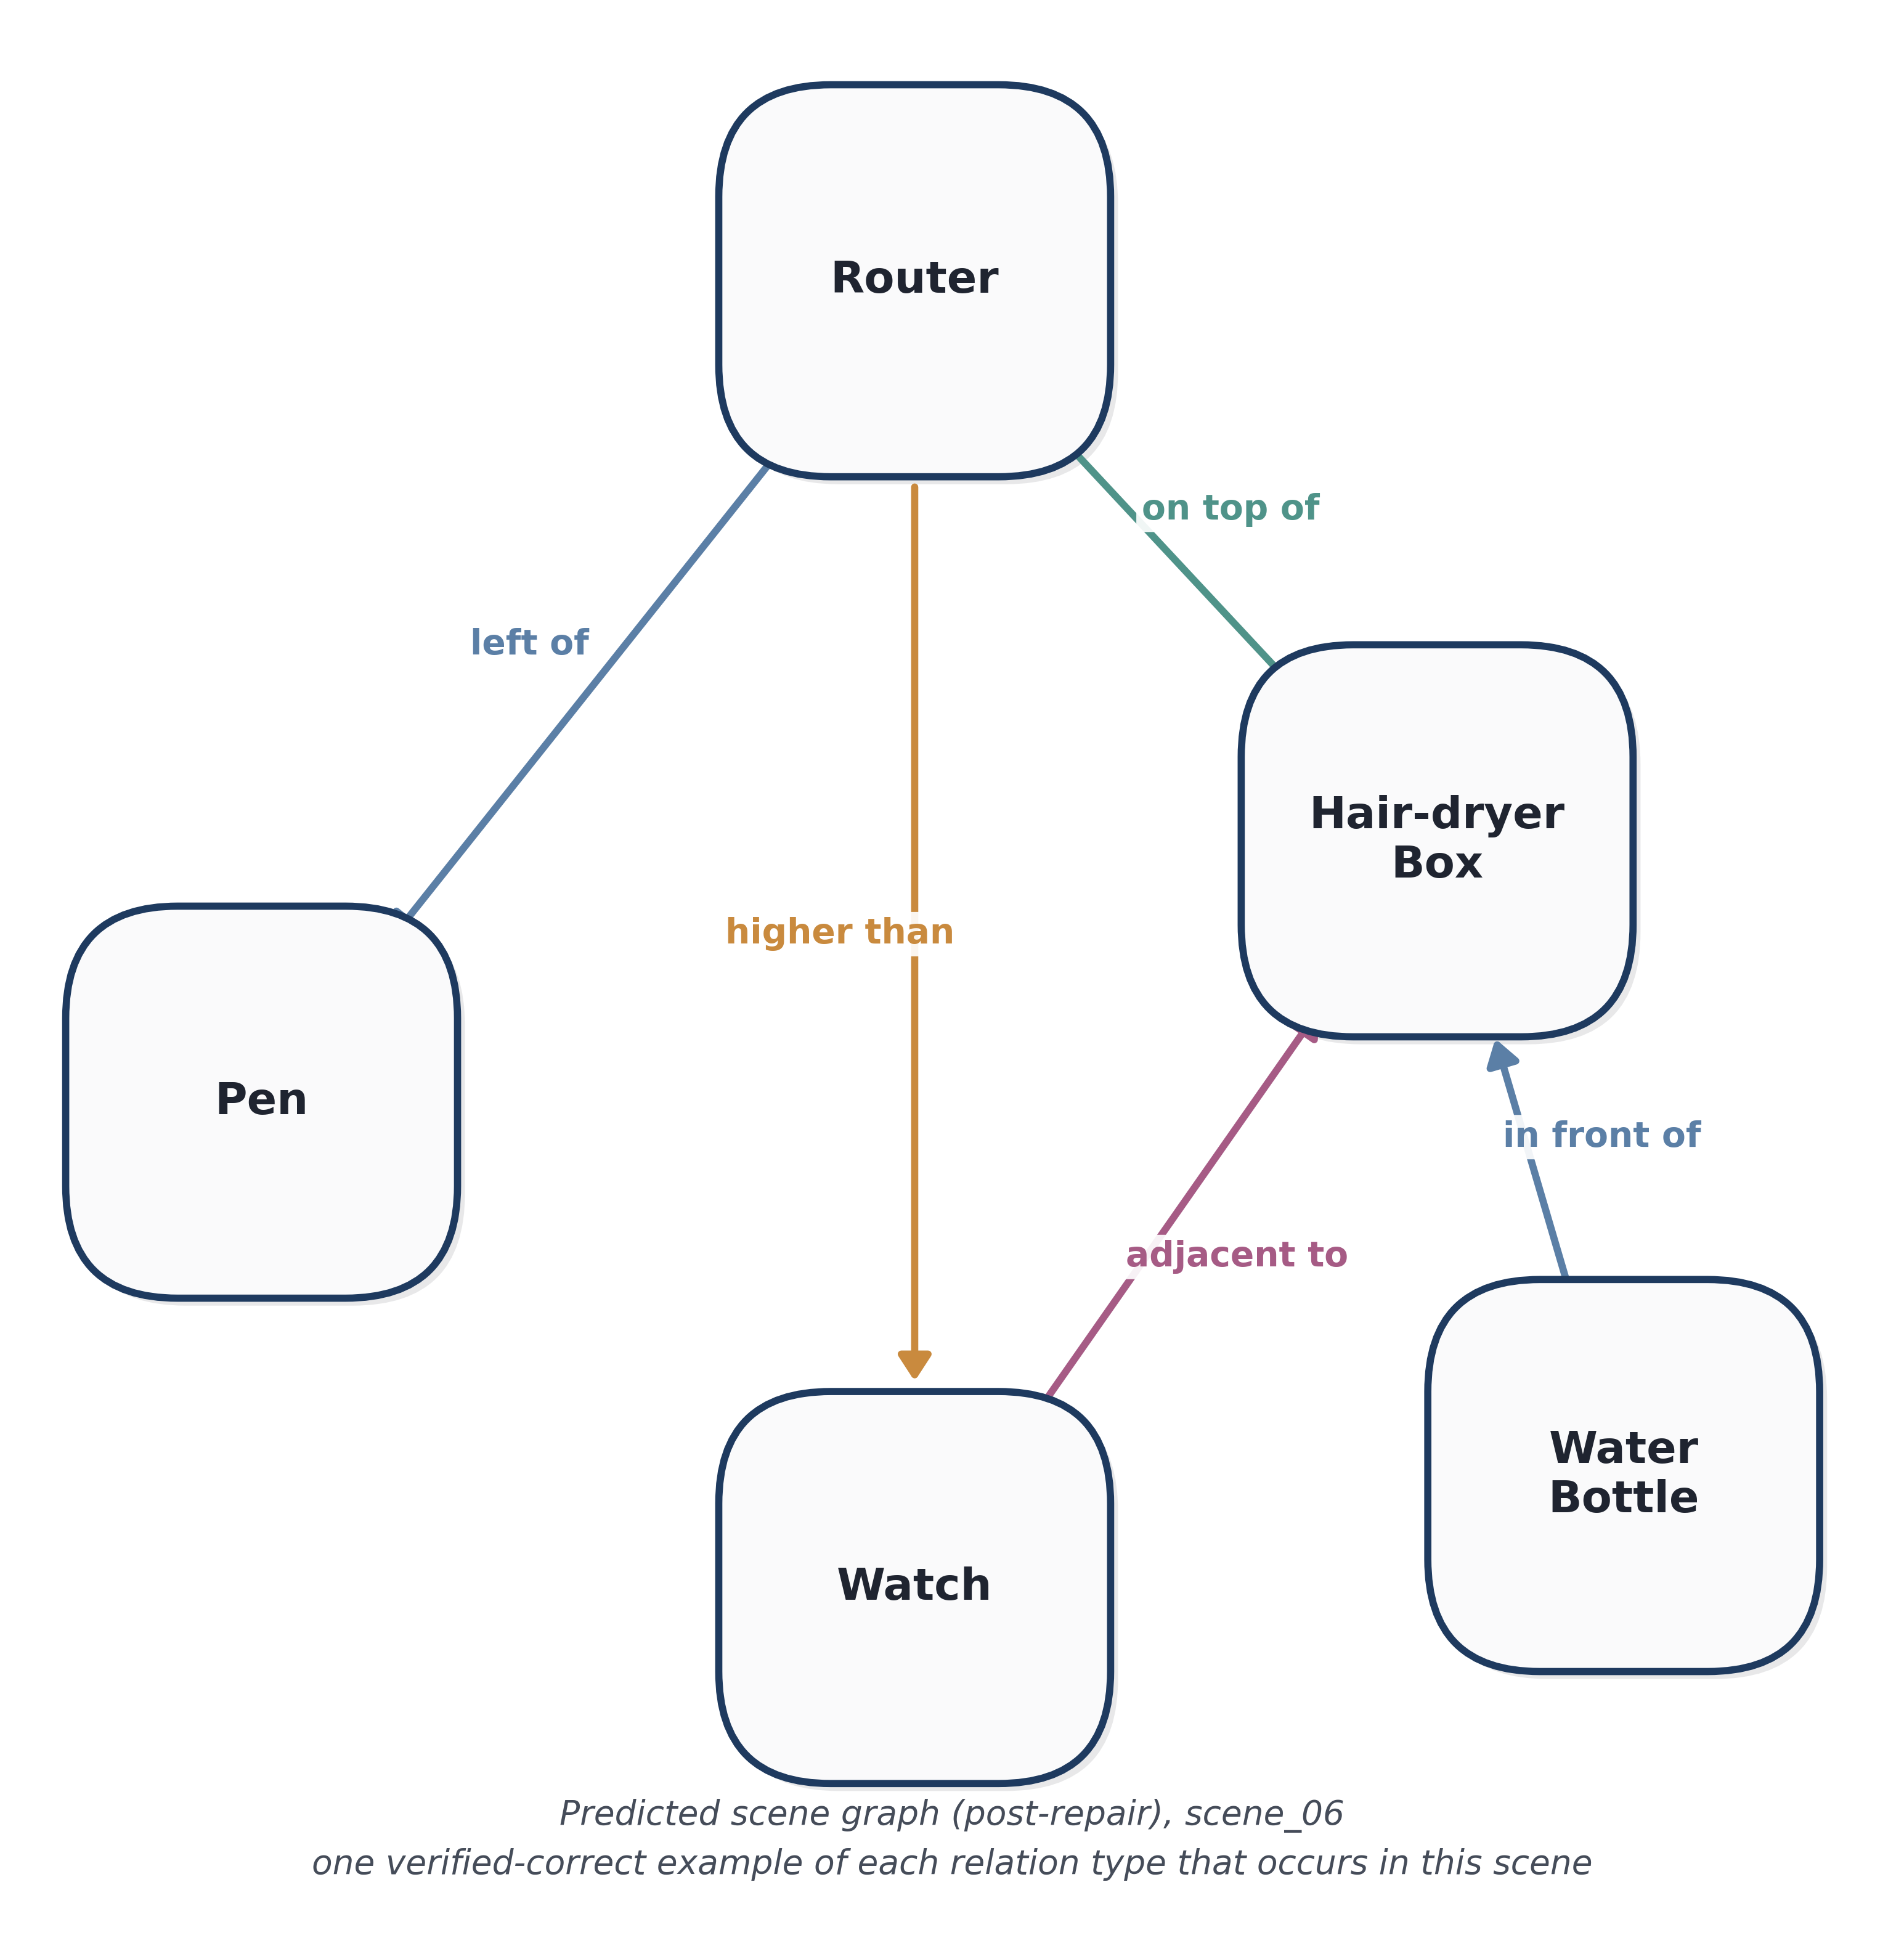
\includegraphics[width=\textwidth]{figures/fig5_qualitative_example.png}
\caption{Predicted scene graph (post-repair) for one tabletop scene, restricted to the five physical objects and a representative, verified-correct subset of predicted relations.}\label{fig7}
\end{figure}

\FloatBarrier
\subsection{Geometric Features as a Sufficient Substitute for Semantic Grounding}\label{subsec5-5}

The results in Sections~\ref{subsec5-1}--\ref{subsec5-4} converge on a claim more specific than ``GeoKAN works'': the spatial relations evaluated here are geometric facts, and a system built around well-engineered, scale-invariant features does not need semantic grounding to predict them accurately --- regardless of which classification head sits on top of that feature design. The matched-budget ablation (Section~\ref{subsec5-1}) reaches Recall@5 = 98.17\% in-distribution, within 0.15 points of GeoKAN-Gamma's 98.32\%, and would itself clear ReLaGS's 87.0\% by essentially the same margin GeoKAN does. The headline claim against foundation-model-dependent systems is therefore a property of the feature design, the rule-based label injection (Section~\ref{subsec4-4}), and the symbolic repair module (Section~\ref{subsec4-8}) --- not of any one architectural choice for the head.

What the architectural choice does determine is how that accuracy survives a change of domain. Across both forms of distribution shift tested in this study --- a scale shift to tabletop scenes an order of magnitude smaller than training (Section~\ref{subsec5-2}) and a dataset shift to an unseen benchmark at comparable scale (Section~\ref{subsec5-3}) --- every GeoKAN configuration tested leads the matched-budget MLP baseline on every reported metric, despite using roughly two-thirds the parameters. On tabletop, where all three basis-function variants were evaluated, the margin ranges from 5.3 to 9.8 Micro F1 points and 4.1 to 5.7 Recall@5 points after repair; on LERF, where Gamma is the variant carried forward (Section~\ref{subsec5-1}), the margin is 2.2 points in both Micro F1 and Recall@5. The direction of this gap holds across two independent held-out settings and across every GeoKAN variant tested cross-domain, which is what distinguishes it from a one-off result: whatever GeoKAN's classification head contributes over a conventional learned layer, it contributes consistently, regardless of which basis function or metric variant is used.

This pattern extends, rather than merely confirms, the recent finding that conventional MLPs match or exceed Kolmogorov-Arnold Networks outside symbolic-regression tasks \cite{yu2024kanmlp}. That comparison was conducted entirely in-distribution; this study's three-setting evaluation adds a dimension it did not test. The cross-domain results also rule out the simplest explanation for why GeoKAN generalises better: a tight, input-independent constraint is not by itself what produces the gain. If it were, Gamma's single fixed scalar per dimension --- the most constrained of the three variants, and the strongest in-distribution (Section~\ref{subsec5-1}) --- should generalise best; instead, on tabletop, it generalises worst of the three, while RBF and Wavelet's input-conditioned MetricNet, the more flexible mechanism, generalises further (Section~\ref{subsec5-2}). What the three variants share, and the MLP baseline lacks, is a metric-warping step at all --- conditioning the basis expansion on a learned notion of which input dimensions matter, rather than learning the expansion directly and unconstrained. Whether that conditioning is a single global scalar or an input-dependent network determines how well the resulting representation survives a change of domain, and on this evidence, conditioning it on the input generalises more reliably than fixing it globally --- an inductive bias that costs nothing in-distribution but pays off precisely where this system is designed to be deployed: outside it.

This efficiency extends to wall-clock cost. Measured on a single consumer laptop GPU, GeoKANRelationGNN's forward pass over a full scene graph completes in 3--4 milliseconds, and symbolic repair adds under 2 milliseconds on top of it, with the network running just as fast on CPU as on GPU for graphs this small --- specialised hardware is a convenience here, not a requirement. The slower stage in the full pipeline is HDBSCAN-based object clustering, at 4.2 to 4.7 seconds per scene, bringing the complete end-to-end pipeline to 5--6 seconds --- still well clear of the over-ten-minutes-per-scene runtimes reported for foundation-model-based systems (Section~\ref{sec1}), with the gap narrowing only because object segmentation, a problem every class-agnostic 3D method shares, is this pipeline's slowest stage rather than relation prediction.

\FloatBarrier
\subsection{Symbolic Repair as Recall Completion}\label{subsec5-6}

Across both held-out evaluation settings, symbolic repair behaves the same way regardless of which GeoKAN variant produced the underlying predictions: it finds few to no contradictions and overwhelmingly adds relations --- a result that speaks well of the network's predictions outside the training distribution, since it indicates they remain largely self-consistent even as raw accuracy degrades under domain shift. The errors that domain shift introduces are concentrated in omission --- relations the network is positioned to recover but does not yet surface above threshold --- rather than in self-contradiction, which is exactly the failure mode this module is designed to address.

Repair's guarantee is, by design, unconditional on logical consistency and conditional on correctness: it completes whatever the network's own predictions imply, and inherits the network's confidence in those predictions rather than independently verifying them. This is what makes it valuable without requiring any additional training data or parameters. On tabletop, this produces a clear, substantial Micro F1 gain for every GeoKAN variant (Section~\ref{subsec5-2}), driven primarily by lower\_than, which improves consistently across all three variants, and by on\_top\_of wherever pre-repair performance leaves room to recover it --- exactly the relations the inverse-completeness and transitive-closure rules are built to act on. On LERF, the same mechanism instead produces a precision/recall trade-off that leaves Micro F1 essentially unchanged: recall rises as genuinely missing relations are completed, while precision falls by a comparable amount as a smaller number of completions inherit an underlying misprediction. Both outcomes follow from the same design choice, applied consistently; which one a given benchmark sees depends on a quantity the module has no way to observe directly --- how often the network's underlying predictions were already correct to begin with.

\FloatBarrier
\subsection{Limitations and Scope}\label{subsec5-7}

The evaluation protocol used in this study reflects a set of deliberate choices about what to isolate at this stage of the work, each leaving a clear, well-defined direction for what comes next. Object instances for the held-out and cross-domain settings are supplied via oracle clustering (Section~\ref{subsec4-9}), the predicate-classification convention standard in 3D scene graph literature, which lets relation-prediction quality --- this study's contribution --- be assessed on its own terms, separately from class-agnostic instance segmentation, a distinct problem with its own dedicated literature. The scenes evaluated span four to thirteen objects, comfortably covering the tabletop-manipulation and single-room scenarios this system targets; extending the evaluation to substantially denser scenes is a natural next step as the approach moves toward larger environments. attached\_to's cross-domain transfer is left to future work, since it does not occur in the tabletop benchmark's natural object arrangements. The comparison against GaussianGraph on LERF rests on ground truth derived from this study's own geometric rule rather than GaussianGraph's LLaVA-based annotation --- the scenes, objects, and relation vocabulary are identical, and the comparison is offered on that basis, with the annotation source stated plainly as a difference in methodology rather than in rigor. Results throughout this study are reported from a single training run per configuration, consistent with the scope of a first systematic comparison across architectures and evaluation settings; extending each comparison to multiple seeds is a natural next step for the closest margins reported here, particularly the in-distribution gap between GeoKAN-Gamma and the matched-budget baseline (Section~\ref{subsec5-1}). The relative contribution of rule-based label injection, the asymmetric loss, and the GeoKAN architecture to the headline result is not separately isolated here --- doing so would require retraining with each mechanism disabled in turn, distinct from the architecture-only comparison in Section~\ref{subsec5-1} --- and is left as a natural extension of the controlled-ablation approach already established in this work.

Finally, the geometric assumptions in Section~\ref{subsec4-3} are designed for static indoor arrangements of rigid objects --- the setting motivating this work's deployment scenarios, from tabletop manipulation to room-scale understanding --- and extending them to dynamic, articulated, or outdoor scenes is a promising direction for future work rather than a requirement of the present design.

\FloatBarrier
\section{Conclusion}\label{sec6}

This study presented LogicSplat, a neuro-symbolic pipeline that predicts ten spatial relation classes directly from 3D Gaussian Splat geometry, without any vision-language model, depth sensor, or semantic label at inference time. Objects are segmented via density-based clustering, represented through scale-invariant geometric features, and classified by GeoKANRelationGNN, whose dual contact/directional heads use Geometric Kolmogorov-Arnold Networks. Rule-based label injection addresses the severe annotation sparsity of the 3DSSG training data, and a zero-parameter symbolic repair module enforces logical consistency on the predicted graph after inference.

On the 3DSSG benchmark, the system achieves Macro F1 = 0.926 and Recall@5 = 98.3\%, exceeding ReLaGS, RelationField, ConceptGraphs, and Open3DSG by 11 to 33 percentage points while using under 0.1\% of the largest baseline's parameters. On four held-out LERF scenes, the system reaches Recall@5 = 95.0\% after symbolic repair, exceeding GaussianGraph's strongest configuration by over 30 percentage points. On eight custom tabletop scenes evaluated zero-shot across an order-of-magnitude scale gap, the system reaches Recall@5 = 92.7\%, with symbolic repair improving Micro F1 by 3.4 points without any retraining. A controlled comparison against a matched-capacity multilayer perceptron shows this advantage over foundation-model-dependent systems is a property of the feature design and training strategy rather than of the classification head alone, while the head itself contributes a measurable generalisation advantage, observed consistently under both scale shift and dataset shift.

Five findings constitute this study's contribution to the field:

\textbf{C1.} Geometry-only spatial relation prediction from Gaussian Splat geometry, with no foundation model at inference time, exceeds every compared foundation-model-dependent or per-scene-optimised method on the 3DSSG benchmark, establishing that semantic grounding is not a prerequisite for geometric spatial reasoning at this task.

\textbf{C2.} Rule-based label injection offers a principled treatment of 3DSSG's annotation sparsity, converting geometrically-certain unannotated pairs into pseudo-labels calibrated to each rule's actual geometric certainty, rather than leaving them as false negatives.

\textbf{C3.} A matched-capacity ablation against a conventional multilayer perceptron shows GeoKAN provides no in-distribution advantage --- consistent with recent findings that Kolmogorov-Arnold Networks generally do not outperform MLPs outside symbolic-regression tasks --- but a consistent generalisation gain under both a scale shift and a dataset shift, extending that literature with a domain-shift axis it had not previously tested.

\textbf{C4.} SceneGraphRepair's value lies in recall completion rather than contradiction removal: across two independent held-out settings, the module's contribution comes almost entirely from completing relations the network under-predicted, indicating that this class of system's out-of-distribution errors are dominated by omission rather than self-contradiction.

\textbf{C5.} Comparing degradation between a dataset shift (LERF) and a scale shift (tabletop) at otherwise comparable difficulty isolates scale, not dataset identity, as the dominant factor in cross-domain transfer for this class of system, with in\_front\_of and behind degrading most under the scale shift and on\_top\_of and lower\_than next.

Future work includes incorporating per-Gaussian covariance features --- planarity, elongation, sphericity --- directly into the node representation, which the splat already encodes but the current feature set does not exploit; extending evaluation to denser scenes and to attached\_to's cross-domain transfer specifically; and testing whether the generalisation advantage identified here for GeoKAN extends to other Kolmogorov-Arnold Network applications under distribution shift more broadly.

\backmatter

\section*{Declarations}

\textbf{Funding:} This research received no external funding from any funding agency, commercial entity, or not-for-profit organization.

\textbf{Conflict of Interest:} The authors declare no competing financial or non-financial interests.

\textbf{Ethics Approval:} This study did not involve human participants, human data, or animal subjects. The custom tabletop scenes used for cross-domain evaluation contain only inanimate household objects; no ethics committee approval was required.

\textbf{Consent to Participate / Consent for Publication:} Not applicable.

\textbf{Data Availability:} The 3RScan and 3DSSG datasets are publicly available from their respective authors under their stated usage agreements. The LERF dataset is publicly available. The custom tabletop scene captures and derived ground-truth annotations generated for this study are available from the corresponding author upon reasonable request.

\textbf{Author Contributions:} Debjyoti Sengupta: conceptualization, methodology, software, data curation, formal analysis, investigation, writing --- original draft. Sahil Shah: supervision, conceptualization, writing --- review and editing.

\begin{thebibliography}{99}
\bibitem{kerbl2023} Kerbl, B., Kopanas, G., Leimk\"uhler, T., Drettakis, G. (2023). 3D Gaussian Splatting for Real-Time Radiance Field Rendering. \textit{ACM Transactions on Graphics} (SIGGRAPH 2023). \href{https://arxiv.org/abs/2308.04079}{arXiv:2308.04079}.

\bibitem{tancik2023} Tancik, M., Weber, E., Ng, E., Li, R., Yi, B., Kerr, J., Wang, T., Kristoffersen, A., Austin, J., Salahi, K., Ahuja, A., McAllister, D., Kanazawa, A. (2023). Nerfstudio: A Modular Framework for Neural Radiance Field Development. \textit{ACM SIGGRAPH 2023}. \href{https://arxiv.org/abs/2302.04264}{arXiv:2302.04264}.

\bibitem{wang2025gaussiangraph} Wang, X., Yang, D., Gao, Y., Yue, Y., Yang, Y., Fu, M. (2025). GaussianGraph: 3D Gaussian-based Scene Graph Generation for Open-world Scene Understanding. \href{https://arxiv.org/abs/2503.04034}{arXiv:2503.04034}.

\bibitem{xie2026relags} Xie, Y., Arafa, A., Javanmardi, A., Millerdurai, C., Hu, J.C., Wang, S., Pagani, A., Stricker, D. (2026). ReLaGS: Relational Language Gaussian Splatting. \textit{CVPR 2026}. \href{https://arxiv.org/abs/2603.17605}{arXiv:2603.17605}.

\bibitem{gu2023conceptgraphs} Gu, Q., Kuwajerwala, A., Morin, S., Jatavallabhula, K.M., Sen, B., Agarwal, A., Rivera, C., Paul, W., Ellis, K., Chellappa, R., Gan, C., de Melo, C.M., Tenenbaum, J.B., Torralba, A., Shkurti, F., Paull, L. (2023). ConceptGraphs: Open-Vocabulary 3D Scene Graphs for Perception and Planning. \href{https://arxiv.org/abs/2309.16650}{arXiv:2309.16650}.

\bibitem{koch2024open3dsg} Koch, S., Vaskevicius, N., Colosi, M., Hermosilla, P., Ropinski, T. (2024). Open3DSG: Open-Vocabulary 3D Scene Graphs from Point Clouds with Queryable Objects and Open-Set Relationships. \textit{CVPR 2024}. \href{https://arxiv.org/abs/2402.12259}{arXiv:2402.12259}.

\bibitem{koch2025relationfield} Koch, S., Wald, J., Colosi, M., Vaskevicius, N., Hermosilla, P., Tombari, F., Ropinski, T. (2025). RelationField: Relate Anything in Radiance Fields. \textit{CVPR 2025}. \href{https://arxiv.org/abs/2412.13652}{arXiv:2412.13652}.

\bibitem{wald2020dsssg} Wald, J., Dhamo, H., Navab, N., Tombari, F. (2020). Learning 3D Semantic Scene Graphs from 3D Indoor Reconstructions. \textit{CVPR 2020}. \href{https://arxiv.org/abs/2004.03967}{arXiv:2004.03967}.

\bibitem{qin2024langsplat} Qin, M., Li, W., Zhou, J., Wang, H., Pfister, H. (2024). LangSplat: 3D Language Gaussian Splatting. \textit{CVPR 2024}. \href{https://arxiv.org/abs/2312.16084}{arXiv:2312.16084}.

\bibitem{ye2024gaussiangrouping} Ye, M., Danelljan, M., Yu, F., Ke, L. (2024). Gaussian Grouping: Segment and Edit Anything in 3D Scenes. \textit{ECCV 2024}. \href{https://arxiv.org/abs/2312.00732}{arXiv:2312.00732}.

\bibitem{cen2025saga} Cen, J., Fang, J., Yang, C., Xie, L., Zhang, X., Shen, W., Tian, Q. (2025). Segment Any 3D Gaussians. \textit{AAAI 2025}. \href{https://arxiv.org/abs/2312.00860}{arXiv:2312.00860}.

\bibitem{wald2019rio} Wald, J., Avetisyan, A., Navab, N., Tombari, F., Niessner, M. (2019). RIO: 3D Object Instance Re-Localization in Changing Indoor Environments. \textit{ICCV 2019}. \href{https://arxiv.org/abs/1908.06109}{arXiv:1908.06109}.

\bibitem{wu2021scenegraphfusion} Wu, S.C., Wald, J., Tateno, K., Navab, N., Tombari, F. (2021). SceneGraphFusion: Incremental 3D Scene Graph Prediction from RGB-D Sequences. \textit{CVPR 2021}. \href{https://arxiv.org/abs/2103.14898}{arXiv:2103.14898}.

\bibitem{velickovic2018gat} Veli\v{c}kovi\'{c}, P., Cucurull, G., Casanova, A., Romero, A., Li\`{o}, P., Bengio, Y. (2018). Graph Attention Networks. \textit{ICLR 2018}. \href{https://arxiv.org/abs/1710.10903}{arXiv:1710.10903}.

\bibitem{brody2022gatv2} Brody, S., Alon, U., Yahav, E. (2022). How Attentive Are Graph Attention Networks? \textit{ICLR 2022}. \href{https://arxiv.org/abs/2105.14491}{arXiv:2105.14491}.

\bibitem{liu2024kan} Liu, Z., Wang, Y., Vaidya, S., Ruehle, F., Halverson, J., Soljacic, M., Hou, T.Y., Tegmark, M. (2024). KAN: Kolmogorov-Arnold Networks. \textit{ICLR 2025}. \href{https://arxiv.org/abs/2404.19756}{arXiv:2404.19756}.

\bibitem{sen2026geokan} Sen, A., Parida, B.K., Maiti, G., Arya, M., Bondar, D.I. (2026). Geometric Kolmogorov-Arnold Network (GeoKAN). \href{https://arxiv.org/abs/2605.06740}{arXiv:2605.06740}.

\bibitem{yu2024kanmlp} Yu, R., Yu, W., Wang, X. (2024). KAN or MLP: A Fairer Comparison. \href{https://arxiv.org/abs/2407.16674}{arXiv:2407.16674}.

\bibitem{ridnik2021asl} Ridnik, T., Ben-Baruch, E., Zamir, N., Noy, A., Friedman, I., Protter, M., Zelnik-Manor, L. (2021). Asymmetric Loss for Multi-Label Classification. \textit{ICCV 2021}. \href{https://arxiv.org/abs/2009.14119}{arXiv:2009.14119}.

\bibitem{wang2020unannotated} Wang, T.J.J., Pehlivan, S., Laaksonen, J. (2020). Tackling the Unannotated: Scene Graph Generation with Bias-Reduced Models. \textit{BMVC 2020}. \href{https://arxiv.org/abs/2008.07832}{arXiv:2008.07832}.

\bibitem{mcinnes2017hdbscan} McInnes, L., Healy, J., Astels, S. (2017). hdbscan: Hierarchical Density-Based Clustering. \textit{Journal of Open Source Software}, 2(11), 205. \href{https://doi.org/10.21105/joss.00205}{https://doi.org/10.21105/joss.00205}.

\bibitem{kerr2023lerf} Kerr, J., Kim, C.M., Goldberg, K., Kanazawa, A., Tancik, M. (2023). LERF: Language Embedded Radiance Fields. \textit{ICCV 2023}. \href{https://arxiv.org/abs/2303.09553}{arXiv:2303.09553}.

\end{thebibliography}

\end{document}
